\renewcommand\chapterillustration{abertura-probabilidade}
\renewcommand\chapterwhat{Reconhecimento de fenômenos determinís-
ticos e aleatórios. Interpretações de proba-
bilidade: clássica, frequentista e subjetiva.

Conceitos básicos. Definição matemática de

probabilidade. Propriedades da probabili-
dade. Probabilidade condicional. Indepen-
dência.}
\renewcommand\chapterbecause{Porque grande parte das decisões científi-
cas de nossa era se dá em ambiente de in-
certeza e a Teoria das Probabilidades é a

área da matemática que fornece estrutu-
ras para a quantificação da aleatoriedade

associada a determinados fenômenos de in-
teresse, para uma tomada de decisão ade-
quada sob incerteza.}
\chapter{Probabilidade}

\mbox{}\thispagestyle{empty}\clearpage

\thispagestyle{empty}

\begin{center}
Projeto: LIVRO ABERTO DE MATEMÁTICA

\noindent \begin{tabular}{lcccr}

\includegraphics[scale=.15]{impa}& \quad\quad& 
\includegraphics[width=3cm]{logo} & \quad\quad& 
\includegraphics[scale=.24]{obmep} 
\end{tabular}
\end{center}

\vspace*{.3cm}

Cadastre-se como colaborador no site do projeto: \url{umlivroaberto.org}

Versão digital do capítulo:

\url{https://www.umlivroaberto.org/BookCloud/Volume_1/master/view/PE511.html}

% \begin{center}
%   \includegraphics[width=2cm]{canvas}
% \end{center}

\begin{tabular}{p{.15\textwidth}p{.7\textwidth}}
Título: & Probabilidade\\
\\
Ano/ Versão: & 2020 / versão 1.0 de 24 de março de 2020\\
\\
Editora & Instituto Nacional de Matem\'atica Pura e Aplicada (IMPA-OS)\\
\\
Realização:& Olimp\'iada Brasileira de Matem\'atica das Escolas P\'ublicas (OBMEP)\\
\\
Produção:& Associação Livro Aberto\\
\\
Coordenação: & Fabio Simas e Augusto Teixeira (livroaberto@impa.br)\\
\\
  Autores: & Flávia Landim (coordenadora da equipe - UFRJ),\\
        & Alexandre Silva (UNIRIO),\\
        & Nei Rocha (UFRJ),\\
             & Vanessa Matos (SEduc Angras dos Reis e Mesquita).\\
\\
Revisora: &  Cydara Ripoll  \\
\\
Design: & Andreza Moreira (Tangentes Design) \\
\\
  Ilustrações: & Miller  Guglielmo \\ 
\\
Gráficos: & Beatriz Cabral e Tarso Caldas (Licenciandos da UNIRIO)\\
\\
  Capa: & Foto de Robert Anasch, no Unsplash \\
        & https://unsplash.com/photos/ugV\_7jiFRxM \\

\end{tabular}

\begin{figure}[b]
\begin{minipage}[l]{5cm}
\centering

{\large Licença:}

  
\includegraphics[width=3.5cm]{cc-by-sa1}
\end{minipage}\hfill
\begin{minipage}[c]{5cm}
\centering
{\large Desenvolvido por}


\includegraphics[width=2.5cm]{logo-associacao.jpg}
\end{minipage}
\begin{minipage}[r]{5cm}
\centering

{\large Patrocínio:}
  \vspace{1em}
  
\includegraphics[width=3.5cm]{itau}
\end{minipage}
\end{figure}

\mainmatter


\explore{conceitos básicos}\label{conceitosbasicos}
Neste capítulo iremos explorar a noção de probabilidade para, em seguida,  apresentar uma teoria matemática útil para calcular probabilidades de \index{eventos}eventos associados a \index{experimentos aleatórios}experimentos aleatórios ou fenômenos aleatórios, isto é, experimentos cujos resultados finais são conhecidos somente após a realização dos mesmos.
Por exemplo,
\begin{enumerate}
\item {} 
o número de \emph{likes} que você irá receber no período de 24h após a sua postagem em uma rede social;

\item {} 
a quantidade de metros cúbicos de gás consumida na sua residência no primeiro semestre do próximo ano ;

\item {} 
o tempo, contado a partir de hoje, que a lâmpada do seu quarto levará para queimar;

\item {} 
o número de quilowatts consumidos na sua residência no próximo mês.

Em contraposição aos fenômenos aleatórios existem os \index{fenômenos determinísticos}fenômenos determinísticos, quando é possível determinar seu resultado mesmo antes de realizá-lo, conhecendo-se determinadas condições. Na natureza existem muitos exemplos de experimentos determinísticos. Por exemplo, na Física há vários modelos determinísticos, como

\item {} 
a primeira lei de Newton que estabelece a força, conhecendo-se massa e aceleração;

\item {} 
a lei do movimento retilíneo uniforme em que é possível calcular a distância percorrida pelo móvel, conhecendo-se a velocidade e tempo transcorrido;

\item {} 
a lei do movimento uniformemente variado em que é possível calcular a distância percorrida pelo móvel, conhecendo-se a aceleração, a velocidade e o tempo transcorrido.

\item {} 
a lei da gravitação universal em que é possível calcular o tempo de queda de um objeto que é lançado em queda livre, conhecendo-se a altura, a aceleração da gravidade, desprezando a resistência do ar.

\end{enumerate}

Tais modelos da Física são chamados modelos matemáticos determinísticos, uma vez que é possível determinar quantidades de interesse, conhecendo-se certas condições, mesmo sem a realização do experimento.

Para explicar fenômenos aleatórios como exemplificados nos itens a) a d), usamos modelos matemáticos não determinísticos chamados modelos probabilísticos. Neste caso, mesmo conhecendo algumas condições, não é possível determinar qual será o resultado antes da realização do experimento.


\subsection{Um pouco de história da Probabilidade}

Antes de começar o estudo um pouco mais formal de probabilidade, apresentaremos um breve resumo sobre a história da probabilidade.

A noção de acaso e ocorrências de fenômenos aleatórios foram percebidas   sensorialmente pela humanidade bem antes de sermos capazes de utilizar a Matemática como forma de descrição do mundo. No entanto, a percepção antiga é de que havia uma razão mítica para o aparecimento de tais fenômenos. Há vários registros históricos de 2700 A.C. do uso de dados antigos (como os ossos astrágalos e dados egípcios, ilustrados nas \hyperref[astragalos]{figuras \ref{astragalos} e \ref{dadosegipcios}}), usados para uma tomada de decisão regida pelos Deuses do Acaso, quando o homem queria se eximir de sua responsabilidade na escolha e tomada de decisão.

\begin{minipage}{0.5\textwidth}
\begin{figure}[H]
\centering
\capstart

\noindent\includegraphics[width=150bp]{{astragalos}.png}
\caption{Astrágalos}\label{astragalos}\end{figure}
\end{minipage}
\begin{minipage}{0.5\textwidth}
\begin{figure}[H]
\centering
\capstart

\noindent\includegraphics[width=150bp]{{dadosegipcios}.png}
\caption{Dados egípcios}\label{dadosegipcios}\end{figure}
\end{minipage}

A própria Bíblia nos informa que  “não cai uma folha de uma árvore sem que o Pai não deseje”. Essa crença de que deuses (no mundo panteísta) ou Deus (no mundo monoteísta) eram os regentes desses fenômenos, acarretou um atraso histórico na matematização do acaso e na criação da Teoria das Probabilidades, uma área considerada cognitivamente desafiadora até hoje na Ciência. Como bem colocou Piaget em seu famoso livro A Origem da Ideia do Acaso na Criança:  “Em contraste com as operações lógicas e aritméticas, a probabilidade é descoberta gradualmente.”

Por isso, foi preciso esperar os séculos XVI e XVII para que matemáticos como Cardano, Tartaglia, Pascal e Fermat (\hyperref[rostos_historia]{figura \ref{rostos_historia}}), para citar alguns, conseguissem dar uma explicação mais consistente do conceito de acaso/aleatoriedade no seio da Matemática, a partir, primordialmente, do estudo de jogos de azar e de sua conexão estreita com a Análise Combinatória.

\begin{figure}[H]
\centering
\capstart

\noindent\includegraphics[width=200bp]{{rostos_historia}.png}
\caption{Alguns matemáticos que originaram a discussão do conceito de acaso}\label{rostos_historia}\end{figure}{}

No entanto, poderíamos dizer que a ideia fundamental por trás da matematização do acaso reside essencialmente na Estatística, quando esta re{}conhece, pela sua{} própria natureza, que fenômenos aleatórios, embora sem explicação determinística, tendem a demonstrar uma certa taxa regular de ocorrência conforme são realizados vários experimentos similares ao longo do tempo. A busca de um modelo que explique tais regularidades de ocorrência do fenômeno em estudo é a ideia central da Teoria das Probabilidades e sua utilidade hoje em vários campos científicos, como Economia, Medicina, Robótica, Engenharia, Computação, Biologia, etc, demonstra como a teoria está mais perto da Estatística do que da abordagem feita por meio do diálogo com a Análise Combinatória durante os Séculos das Luzes.

É somente na primeira metade do século XX que a teoria das probabilidades vai adquirir uma base axiomática rigorosa por meio da construção teórica estabelecida pelo matemático russo Kolmogorov (\hyperref[kolmogorov]{figura \ref{kolmogorov}}). Desde então a teoria das probabilidades tem sido vista como uma das áreas mais promissoras da Matemática e a ferramenta por excelência para modelar e explicar os mais variados fenômenos aleatórios presentes no mundo contemporâneo.

\begin{figure}[H]
\centering
\capstart

\noindent\includegraphics[width=150bp]{{kolmogorov}.png}
\caption{Andrei Kolmogorov}\label{kolmogorov}\end{figure}

Veja na \hyperref[linhadotempo]{figura \ref{linhadotempo}} uma linha do tempo destacando acontecimentos importantes no desenvolvimento da teoria das probabilidades.

\begin{figure}[H]
\centering
\capstart
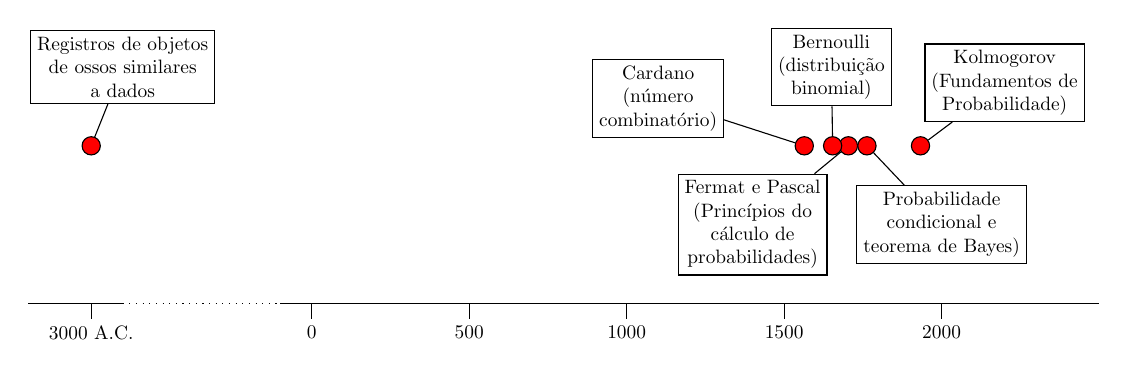
\begin{tikzpicture}[scale=.4, every node/.style={scale=.7}]
     \tikzstyle{quadro}=[rectangle,draw, minimum width=1cm, minimum height=0.5, align=left]
         \tikzstyle{circulo}=[circle, draw, minimum size=0.05cm, fill=red]
         
         \draw (-9,-.5) -- (-6,-.50);
         \draw (-1,-.5) -- (0,-.5) -- (25,-.5);
         \draw [dotted] (-6,-.5) -- (-1,-.5);
         \foreach \x/\y in {-7/3000 A.C.,0/0,5/500,10/1000,15/1500,20/2000} \draw (\x,-0.5) -- (\x,-1) node [below] {\y};

         \node (qRegistros) at (-6,7) [quadro,align=center] {Registros de objetos \\ de ossos similares \\ a dados};
         \node (qCardano) at (11,6) [quadro, align=center] {Cardano \\ (número \\ combinatório)};
         \node (qFermat) at (14,2) [quadro,align=center] {Fermat e Pascal \\ (Princípios do \\ cálculo de \\ probabilidades)};
         \node (qBernoulli) at (16.5,7) [quadro,align=center] {Bernoulli \\ (distribuição \\ binomial)};
         \node (qBayes) at (20,2) [quadro,align=center] {Probabilidade \\ condicional e \\ teorema de Bayes)};
         \node (qKolmogorov) [quadro,align=center] at (22,6.5) {Kolmogorov \\ (Fundamentos de \\ Probabilidade)};
         
         
         \node (registros) at  (-7,4.5) [circulo] {};
         \node (Cardano) at  (15.64,4.5) [ circulo] {};
         \node (Fermat) at (17.04,4.5) [circulo] {};
         \node (Bernoulli) at (16.54,4.5) [circulo] {};
         \node (Bayes) at (17.63,4.5) [circulo] {};
         \node (Kolmogorov)  at(19.33,4.5) [circulo] {};
         
         \path
         (registros) edge (qRegistros)
         (Cardano) edge (qCardano)
         (Fermat) edge (qFermat)
         (Bernoulli) edge (qBernoulli)
         (Bayes) edge (qBayes)
         (Kolmogorov) edge (qKolmogorov);
\end{tikzpicture}
\caption{Linha do tempo}\label{linhadotempo}
\end{figure}

Nos capítulos \textbf{A Natureza da Estatística} e \textbf{Medidas de Posição e Dispersão}, vimos como resumir a informação de dados aleatórios amostrais com o objetivo de  entender estruturas úteis para uma tomada de decisão sob incerteza. Neste capítulo, analisaremos as características extraídas dos dados aleatórios amostrais a fim de revelar como a Estatística nos auxilia a descrever as regularidades de ocorrências de determinados eventos aleatórios.
\pagebreak

\begin{task}{não determinístico (aleatório) ou determinístico?}

Classifique cada experimento a seguir em aleatório ou determinístico.

Deseja-se observar:
\begin{enumerate}[rightmargin=3mm]
\item 
o valor constante de cada prestação quando se financia um eletrodoméstico, estabelecendo-se a taxa de juros efetiva ao mês, a quantidade de meses do financiamento e o pagamento da primeira prestação no ato da compra.

\item 
a distância percorrida por um objeto em movimento, conhecendo-se a velocidade e o tempo transcorrido.

\item 
a quantidade de metros cúbicos de água consumida em sua residência no primeiro semestre do próximo ano.

\item 
o valor a ser pago na conta de luz da sua residência no próximo mês.

\item 
a sua média final em Matemática desse ano.

\end{enumerate}
\end{task}
\begin{task}{interpretando medida de incerteza}


Responda os itens a seguir.
\begin{enumerate}
\item {} 
A probabilidade de ocorrer cara quando lançamos uma moeda honesta é 0,5. Isso significa que toda vez que lançarmos essa moeda 100 vezes, ocorrerão 50 caras? Por quê?

\item {} 
Foi publicada a previsão do tempo, indicando que a probabilidade de chover amanhã na região onde você mora e estuda é de 30{}`\%{}`. Que decisão você tomaria com base nessa previsão: levar ou não um guarda-chuva para a escola? Por quê? Como você interpreta essa previsão?

\item {} 
Um estudo na área de Saúde indicou que a probabilidade de uma pessoa vir a ter o Diabetes é 10{}`\%{}`. Isso significa que ao acompanhar um grupo de 500 pessoas, 50 delas terão Diabetes? Por quê?

\end{enumerate}
\end{task}
\begin{task}{avaliando probabilidades}


Bloco I - Probabilidade clássica
\begin{enumerate}
\item {} 
De um grupo de 10 estudantes, um será sorteado para ser o representante de turma. Como são 4 meninas e seis meninos, decidiu-se, para fazer o sorteio,  representar as meninas por cartões ilustrados com triângulos e os meninos por cartões ilustrados com círculos. Os cartões foram colocados numa caixa e um será sorteado (\hyperref[cartoesilustrados]{figura \ref{cartoesilustrados}}).

\begin{figure}[H]
\centering

\begin{tikzpicture}
[scale=0.6]
\draw [,rounded corners=8pt, -] (0,-0) -- (0,10) -- (10,10) -- (10,0) -- cycle;
       \draw (0.25,6.5) rectangle (1.75,8.5);
       \draw (2.25,6.5) rectangle (3.75,8.5);
       \draw (4.25,6.5) rectangle (5.75,8.5);
       \draw (6.25,6.5) rectangle (7.75,8.5);
       \draw (8.25,6.5) rectangle (9.75,8.5);
       \draw (0.25,1.5) rectangle (1.75,3.5);
       \draw (2.25,1.5) rectangle (3.75,3.5);
       \draw (4.25,1.5) rectangle (5.75,3.5);
       \draw (6.25,1.5) rectangle (7.75,3.5);
       \draw (8.25,1.5) rectangle (9.75,3.5);
       \draw [color=primario, fill=primario] (1,7.5) circle (12pt);
       \draw [color=primario, fill=primario] (5,7.5) circle (12pt);
       \draw [color=primario, fill=primario] (7,7.5) circle (12pt);
       \draw [color=primario, fill=primario] (3,2.5) circle (12pt);
       \draw [color=primario, fill=primario] (5,2.5) circle (12pt);
       \draw [color=primario, fill=primario] (9,2.5) circle (12pt);
       \draw [color=atento, fill=atento, rounded corners=1pt, -] (3,8) -- (3.5,7) -- (2.5,7) -- (3,8) --  cycle;
       \draw [color=atento, fill=atento, rounded corners=1pt, -] (9,8) -- (9.5,7) -- (8.5,7) -- (9,8) --  cycle;
\draw [color=atento, fill=atento, ] (1,3) -- (1.5,2) -- (.5,2) -- (1,3) --  cycle;
       \draw [color=atento, fill=atento] (7,3) -- (7.5,2) -- (6.5,2) -- (7,3) --  cycle;
\end{tikzpicture}
\caption{Cartões ilustrados}
\label{cartoesilustrados}
\end{figure}

Qual é a probabilidade (chance) de ser escolhida uma menina como representante de turma? Por quê?

\item {} 
Numa rua há 10 casas. O número de moradores por casa está representado na \hyperref[moradorescasa]{figura \ref{moradorescasa}}. Suponha que você irá escolher ao acaso uma casa desta rua.
\begin{figure}[H]
\centering

\begin{tikzpicture}
\begin{scope}[scale=.6]
\draw  [color = terciario, fill =terciario](0.25,6.5) rectangle (1.25,8.5);
\draw [color = terciario, fill =terciario](2.25,6.5) rectangle (3.25,8.5);
\draw [color = terciario, fill =terciario](4.25,6.5) rectangle (5.25,8.5);
\draw [color = terciario, fill =terciario](6.25,6.5) rectangle (7.25,8.5);
\draw [color = terciario, fill =terciario](8.25,6.5) rectangle (9.25,8.5);
\draw [fill = destacado!50, color=destacado!50,-] (1.4,8.5) -- (.05,8.5) -- (.73,9.5) -- cycle;
\draw [fill = destacado!50, color=destacado!50,-] (3.4,8.5) -- (2.05,8.5) -- (2.73,9.5) -- cycle;
\draw [fill = destacado!50, color=destacado!50,-] (5.4,8.5) -- (4.05,8.5) -- (4.73,9.5) -- cycle;
\draw [fill = destacado!50, color=destacado!50,-] (7.4,8.5) -- (6.05,8.5) -- (6.73,9.5) -- cycle;
\draw [fill = destacado!50, color=destacado!50,-] (9.4,8.5) -- (8.05,8.5) -- (8.73,9.5) -- cycle;
\draw [color = terciario, fill =terciario](0.25,1.5) rectangle (1.25,3.5);
\draw [color = terciario, fill =terciario](2.25,1.5) rectangle (3.25,3.5);
\draw [color = terciario, fill =terciario](4.25,1.5) rectangle (5.25,3.5);
\draw [color = terciario, fill =terciario](6.25,1.5) rectangle (7.25,3.5);
\draw [color = terciario, fill =terciario](8.25,1.5) rectangle (9.25,3.5);
\draw [fill = destacado!50, color=destacado!50,-] (1.4,3.5) -- (.05,3.5) -- (.73,4.5) -- cycle;
\draw [fill = destacado!50, color=destacado!50,-] (3.4,3.5) -- (2.05,3.5) -- (2.73,4.5) -- cycle;
\draw [fill = destacado!50, color=destacado!50,-] (5.4,3.5) -- (4.05,3.5) -- (4.73,4.5) -- cycle;
\draw [fill = destacado!50, color=destacado!50,-] (7.4,3.5) -- (6.05,3.5) -- (6.73,4.5) -- cycle;
\draw [fill = destacado!50, color=destacado!50,-] (9.4,3.5) -- (8.05,3.5) -- (8.73,4.5) -- cycle;
\node at (.75,2.5) {1};
\node at (2.75,2.5) {1};
\node at (4.75,2.5) {3};
\node at (6.75,2.5) {2};
\node at (8.75,2.5) {6};
\node at (.75,7.5) {5};
\node at (2.75,7.5) {4};
\node at (4.75,7.5) {8};
\node at (6.75,7.5) {8};
\node at (8.75,7.5) {4};
\end{scope}
\end{tikzpicture}
\caption{Ilustração dos números de moradores por casa}
\label{moradorescasa}
\end{figure}

\item {} 
Qual é a probabilidade de que a casa escolhida tenha exatamente 4 moradores? Por quê?

\item {} 
Qual é a probabilidade de que a casa escolhida tenha mais de 4 moradores? Por quê?

\item {} 
Suponha que você vá girar a roleta ilustrada na \hyperref[roleta]{figura \ref{roleta}}.

\begin{figure}[H]
\centering

\begin{tikzpicture}  

  
  \draw[fill=\currentcolor!70, smooth] (0,0) -- +(90:3) arc (90:180:3cm);
  \draw (0,0) -- (-3,0);
  \draw [thick](0,0) circle (3cm); 
  \draw (-.5,0) -- (-.5,.5) -- (0,.5);
  \draw [fill = black, smooth] (-.25,.25) circle (1pt);
  \draw [->] (1,-1.2) arc (0:-100:.75cm);
  \draw [thick, ->] (0,0) -- (2,-2);
  \draw [color=destacado, fill = destacado] (0,0) circle (.1cm);

\end{tikzpicture}
\caption{Roleta}
\label{roleta}
\end{figure}


\end{enumerate}

Qual é a probabilidade de que a seta pare na região pintada de cinza? Por quê?

Bloco II - Probabilidade frequentista
\begin{enumerate}
\item {} 
Suponha que você tenha lançado uma moeda 20 vezes e que tenha observado a face “cara” 19 vezes e a face “coroa” uma vez. Se você lançar esta moeda mais uma vez, qual é a probabilidade (chance) de a face voltada para cima resultar em “cara”? Por quê?

\item {} 
Suponha que um bebê tenha nascido na maternidade mais próxima de sua casa na manhã de hoje. Qual é a probabilidade de que este bebê seja um menino? Por quê?

\item {} 
A pesquisa TIC Educação 2016, do Centro de Estudos sobre as Tecnologias da Informação e da Comunicação (Cetic), coletou dados de cerca de 11 mil estudantes do segundo segmento do Ensino Fundamental e do Ensino Médio. Entre várias informações, verificou-se que cerca de 8.500 estudantes usam smartphones como seu principal meio de acesso à internet. A pesquisa aconteceu entre agosto e dezembro de 2016.” (\href{https://g1.globo.com/educacao/noticia/52-das-instituicoes-de-educacao-basica-usam-celular-em-atividades-escolares-aponta-estudo-da-cetic.ghtml}{Leia a reportagem} publicada no G1.com.br).

\end{enumerate}

Qual é a probabilidade de que um estudante de Ensino Fundamental II ou Médio, escohido ao acaso, use como seu principal meio de acesso à internet um smartphone, usando os dados dessa pesquisa? Por quê?

Bloco III - Probabilidade subjetiva
\begin{enumerate}
\item {} 
Qual é a probabilidade de que o Brasil se classifique na fase de grupos na próxima Copa do Mundo que irá competir?

\item {} 
Qual é a probabilidade de que daqui a 8 anos você tenha concluído um curso de nível superior?

\item {} 
Qual é a probabilidade de que você esteja casado(a) aos 25 anos?

\end{enumerate}
\end{task}


\arrange{conceitos básicos}
\label{organizandoconceitosbasicos}
Como você fez para determinar as probabilidades no bloco I da Atividade \emph{avaliando probabilidades}? E no bloco II? E no bloco III? Você deve ter percebido que, dependendo da situação, nem sempre é possível atribuir probabilidades a um evento, usando o mesmo tipo de raciocínio.

Por exemplo, considere o experimento “observar se um corpo celeste cairá sobre a casa onde você mora dentro de uma hora”.

\begin{figure}[H]
\centering

\noindent\includegraphics[width=200bp]{{corpoceleste}.png}
\caption{Corpo celeste}
\end{figure}


Há dois resultados possíveis: cair ou não cair. Você acha que é razoável atribuir probabilidades iguais a estes dois resultados?

Certamente não, pois sabemos que a situação “cair” é um evento raríssimo. Em toda a sua vida, você já observou um evento deste tipo?

Neste caso, não faz sentido atribuir probabilidades iguais para os dois resultados possíveis. Uma probabilidade razoável para o resultado “cair” seria bem pequena, próxima de zero e não igual a probabilidade do resultado “não cair”.

Antes de apresentarmos diferentes interpretações de probabilidade, vamos começar definindo os termos \index{espaço amostral}espaço amostral e \index{evento}evento.
\begin{description}
\item[{Espaço amostral \index{Espaço amostral: conjunto que compreende todos os resultados possíveis de um experimento aleatório.|textbf}}]
Conjunto que compreende todos os resultados possíveis de um experimento aleatório.
\end{description}

Usaremos a letra maiúscula \(S\) para denotar espaço amostral.

Por exemplo, no item (b), do bloco I da Atividade \emph{avaliando probabilidades}, um espaço amostral pode ser representado por \(S=\{1,2,3,4,5,6,8\}\), pois este conjunto compreende todos os números possíveis de serem obtidos, quando sorteamos uma casa do bairro. Observe novamente que, neste caso, também não é razoável atribuir probabilidades iguais aos elementos deste espaço amostral, pois na rua há duas casas com exatamente 1 morador, duas casas com exatamente 4 moradores e duas casas com exatamente 8 moradores, enquanto que há apenas uma casa com exatamente 2 moradores, uma casa com  exatamente 3 moradores, uma casa com exatamente 5 moradores e uma casa com exatamente 6 moradores.
\begin{description}
\item[{Evento \index{Evento: é qualquer subconjunto  do espaço amostral  para o qual faz sentido atribuir uma probabilidade.|textbf}}]
É qualquer subconjunto \(A\) do espaço amostral \(S\) para o qual faz sentido atribuir uma probabilidade.
\end{description}

Veja, na \hyperref[diagramavenn1]{figura \ref{diagramavenn1}}, uma representação de um evento (conjunto) \(A\) em um espaço amostral \(S\) (conjunto universo), usando diagrama de Venn.
\begin{figure}[H]
\centering

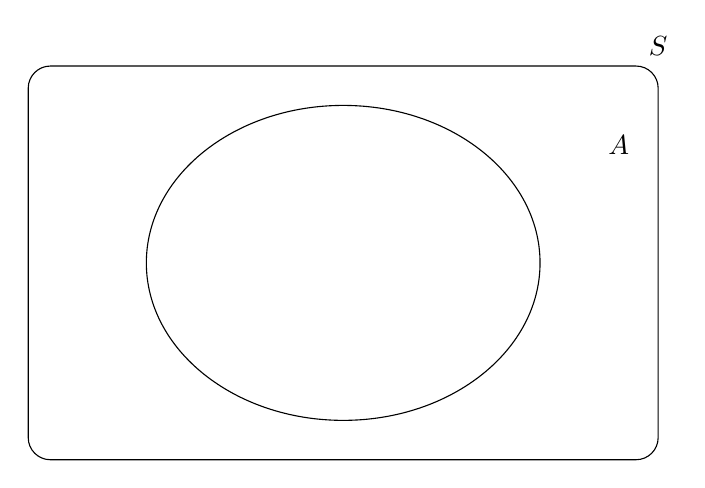
\begin{tikzpicture}

[scale=0.6]
\draw [,rounded corners=8pt, -] (0,-0) -- (0,5) -- (8,5) -- (8,0) -- cycle;
\draw (4,2.5) ellipse (2.5cm and 2cm);
\node [] at (7.5,4) {$A$};
\node [] at (8,5.25) {$S$};
\end{tikzpicture}
\caption{Representação de conjuntos no diagrama de Venn}
\label{diagramavenn1}
\end{figure}

Ao realizar um experimento aleatório, dizemos que um evento \(A\) ocorreu, se o resultado tiver sido um elemento de \(A\). Por exemplo, se ao lançarmos um dado com as faces numeradas de 1 a 6, tiver ocorrido face 2 e \(A\) é o evento “a face voltada para cima corresponde a um número par”, isto é, \(A=\{2,4,6\}\), dizemos que o evento \(A\) ocorreu.

\begin{figure}[H]
\centering

\noindent\includegraphics[width=200bp]{{dados}.png}
\caption{Dados comuns de seis faces numeradas de 1 a 6}
\end{figure}

\begin{description}
\item[{Evento elementar\index{Evento elementar: subconjunto unitário do espaço amostral !ou, equivalentemente, subconjunto do espaço amostral  no qual há apenas um resultado possível.|textbf}}]
Subconjunto unitário do espaço amostral \(S\); ou, equivalentemente, subconjunto do espaço amostral \(S\) no qual há apenas um resultado possível.
\end{description}

Por exemplo, no lançamento de um dado, podemos representar o espaço amostral por \(S=\{1,2,3,4,5,6\}\). Nesse caso, os eventos elementares são os conjuntos unitários:
\begin{equation*}
\begin{split}\{1\}, \{2\}, \{3\}, \{4\}, \{5\} \textsf{ e } \{6\}.\end{split}
\end{equation*}
\textbf{Operações de união, interseção e complementariedade}

Faremos agora uma rápida revisão sobre operações entre conjuntos (união, interseção e complementariedade), pois eventos são conjuntos e nós estamos interessados em calcular probabilidades de eventos.

\begin{description}
  \item[{União}] O conjunto \(A\cup B\) (lê-se \(A\)  união \(B\)) corresponde à reunião de todos os elementos de \(A\) e {}` de \(B\). Veja na \hyperref[aub]{figura \ref{aub}}, uma representação de \(A\cup B\), usando diagrama de Venn, em que o conjunto \(A\cup B\) corresponde à região pintada.

\begin{figure}[H]
\centering

\begin{tikzpicture}  

[scale=0.6, every node/.style={scale=0.6}]
\draw [rounded corners=8pt, -] (0,-0) -- (0,5) -- (8,5) -- (8,0) -- cycle;

\node at (7,4) {$B$};
\node at (.5,4) {$A$};
\node at (7,5.25) {$S$};
\draw [fill=\currentcolor!80, smooth] (5,2.5) circle (2cm);

\draw [fill=\currentcolor!80, smooth] (2.5,2.5) circle (2cm);
\clip [draw] (2.5,2.5) circle (2cm);
\draw [fill= \currentcolor!80, smooth] (5,2.5) circle (2cm);


\end{tikzpicture}
\caption{\(A\cup B\)}
\label{aub}
\end{figure}


Dizemos que o evento \(A\cup B\) ocorreu se pelo menos um dos dois eventos, \(A\) ou \(B\), tiver ocorrido.
\end{description}
\begin{description}
\item [{Interseção}] 
O conjunto \(A\cap B\) (lê-se \(A\) interseção \(B\)) corresponde à coleção de todos os elementos que pertencem simultaneamente ao conjunto \(A\) e ao conjunto \(B\). Veja na \hyperref[intersecao]{figura \ref{intersecao}} uma representação de \(A\cap B\), usando diagrama de Venn, em que o conjunto \(A\cap B\) corresponde à região pintada.
\begin{figure}[H]
\centering

\begin{tikzpicture}

[scale=0.6]
\draw [,rounded corners=8pt, -] (0,-0) -- (0,5) -- (8,5) -- (8,0) -- cycle;
\node at (7,4) {$B$};
\node at (.5,4) {$A$};
\node at (7,5.25) {$S$};
\draw (5,2.5) circle (2cm);
\clip [draw] (2.5,2.5) circle (2cm);
\draw [fill=\currentcolor!80] (5,2.5) circle (2cm);
\end{tikzpicture}
\caption{\(A\cap B\)}
\label{intersecao}
\end{figure}


Dizemos que o evento \(A \cap B\) ocoreu, se os eventos \(A\) e \(B\) tiverem ocorrido simultaneamente.
\end{description}
\begin{description}
\item [{Complementariedade}]
O conjunto \(\overline{A}\) (lê-se \(A\) complementar) corresponde à coleção de todos os elementos do conjunto universo (espaço amostral \(S\)) que não pertencem ao conjunto \(A\). Veja na \hyperref[complementar]{figura \ref{complementar}} uma representação de \(\overline{A}\), usando diagrama de Venn, em que o conjunto \(\overline{A}\) corresponde à região pintada.

\begin{figure}[H]
\centering

\begin{tikzpicture}
\draw [,fill=\currentcolor!80,rounded corners=8pt, -] (0,-0) -- (0,5) -- (8,5) -- (8,0) -- cycle;
\node at (7,4) {$\overline{A}$};
\node at (.5,4) {$A$};
\node at (7,5.25) {$S$};
\draw[fill=white] (2.5,2.5) circle (2cm);
\end{tikzpicture}
\caption{Evento complementar de \(A: \overline{A}\)}
\label{complementar}
\end{figure}

Dizemos que o evento \(\overline{A}\) ocorreu, se o evento \(A\) não tiver ocorrido.
\end{description}

Pela definição das operações de união, interseção e complementareidade dizemos que
\begin{itemize}
\item {} 
o evento \(A\cup B\)  ocorreu se, e somente se, pelo menos um dos dois eventos \(A\) ou \(B\) tiverem ocorrido;

\item {} 
o evento \(A\cap B\) ocorreu se, e somente se, os dois eventos \(A\) e \(B\) tiverem ocorrido simultanemante.

\item {} 
o evento \(\overline{A}\) ocorreu se, e somente se, o evento \(A\) \textbf{não} tiver ocorrido.

\end{itemize}

\begin{description}
\item[{Dois eventos \(A\)  e \(B\) são ditos eventos disjuntos se\index{Dois eventos   e  são ditos (eventos) disjuntos se , ou seja, se  e  não tiverem elementos em comum.|textbf}}]
$A\cap B=\emptyset$, ou seja, se \(A\) e \(B\) não tiverem elementos em comum.
\end{description}

Dado qualquer espaço amostral \(S\), os conjuntos \(S\) e \(\emptyset\) (conjunto vazio) são considerados eventos especiais e chamados de \textbf{evento certo} e \textbf{evento impossível}, respectivamente.

Para o evento certo (\(S\)) atribui-se probabilidade 1 e, para o evento impossível (\(\emptyset\)), atribui-se probabilidade zero. Para qualquer outro evento, a probabilidade deverá ser um número real no intervalo {[}0,1{]}.

Para concluir essa breve revisão de operações com conjuntos, vamos apresentar a propriedade distributiva da operação de interseção com a união de dois eventos, a saber,

\begin{equation*}
\begin{split}(A\cup B)\cap C=(A\cap C)\cup (B\cap C)\end{split}
\end{equation*}

Para visualizar melhor essa propriedade, considere A, B e C eventos em um espaço amostral S, representados nos diagramas de Venn da \hyperref[diagramasvenn2]{figura \ref{diagramasvenn2}}, lembrando que as interseções nesses diagramas podem ser conjuntos vazios.

\begin{figure}[H]
\centering
\begin{minipage}{0.35\textwidth}
\centering
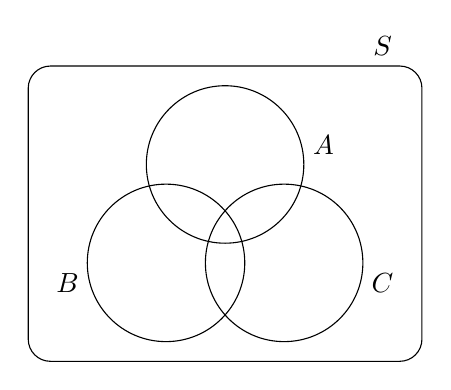
\begin{tikzpicture}[scale=0.5, every node/.style={scale=1}]
\draw [,rounded corners=8pt,] (0,0) -- (0,7.5) -- (10,7.5) -- (10,0) -- cycle;
\node  at (9,8) {$S$};
\draw (3.5,2.5) circle (2cm);
\node  at (1,2) {$B$};
\draw (6.5,2.5) circle (2cm);
\node  at (9,2) {$C$};
\draw (5,5) circle (2cm);
\node  at (7.5,5.5) {$A$};
\end{tikzpicture}

\end{minipage}
\begin{minipage}{0.35\textwidth}
\centering
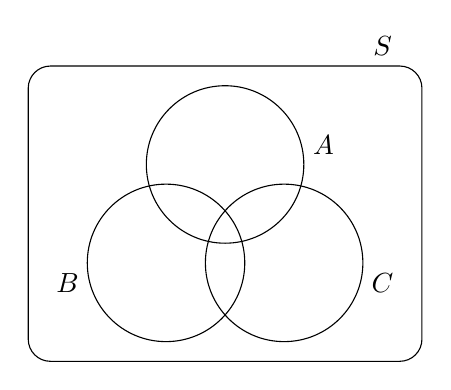
\begin{tikzpicture}[scale=0.5, every node/.style={scale=1}]

\draw [,rounded corners=8pt,] (0,0) -- (0,7.5) -- (10,7.5) -- (10,0) -- cycle;
\node at (9,8) {$S$};
\draw (3.5,2.5) circle (2cm);
\node at (1,2) {$B$};
\draw (6.5,2.5) circle (2cm);
\node at (9,2) {$C$};
\draw (5,5) circle (2cm);
\node at (7.5,5.5) {$A$};
\end{tikzpicture}

\end{minipage}
\caption{Diagramas de Venn com três conjuntos: \(A\), \(B\)  e \(C\)}
\label{diagramasvenn2}
\end{figure}




No primeiro diagrama, pinte de uma cor \(A\cup B\) e com outra cor, pinte o conjunto \(C\), destacando a região que foi pintada pelas duas cores. No segundo diagrama, pinte o conjunto \(A\cap C\) e, com a mesma cor,  o conjunto \(B\cap C\). A região pintadada corresponde ao conjunto dado no lado direito da igualdade. Finalmente, verifique que as regiões destacadas correspondem ao mesmo conjunto.

A seguir, serão apresentadas três interpretações da probabilidade.


\subsection{Interpretação clássica de probabilidade}

Na \index{interpretação clássica de probabilidade}interpretação clássica de probabilidade todos os eventos elementares são considerados igualmente prováveis (equiprováveis).

Esta interpretação costuma ser usada em problemas envolvendo lançamento de dados,  sorteios de cartas de um baralho e outros jogos. De fato, os primeiros trabalhos teóricos publicados envolvendo probabilidades no século XVII, fazem uso desta interpretação e envolvem cálculos de probabilidades de eventos em jogos de azar.

No entanto, nem sempre a interpretação clássica será adequada: lembre-se do exemplo da queda de um corpo celeste.

Um outro problema com esta interpretação é a circularidade do conceito de probabilidade para definir a própria probabilidade, pois considera em sua definição “resultados igualmente prováveis” que depende do conceito de probabilidade.


\subsection{Interpretação frequentista de probabilidade}

Na \index{interpretação frequentista de probabilidade}interpretação frequentista de probabilidade, a probabilidade de um evento é definida como a frequência relativa de ocorrência deste evento, se o experimento for repetido, sob as mesmas condições, um grande número de vezes.

Problemas com esta definição envolvem falta de clareza: o que siginificam
\begin{itemize}
\item {} 
“sob as mesmas condições”? e

\item {} 
“um grande número de vezes”?

\end{itemize}

Além disso, existem fenômenos únicos para os quais não é possível realizar repetições, por exemplo, o experimento que envolve verificar se daqui a 8 anos seu nível de instrução será superior completo ou não.

No entanto, esta interpretação é muito útil e amplamente usada em modelagens probabilísticas. De fato, a interpretação frequentista de probabilidade tem suas origens com a Lei dos Grandes Números, importante resultado da teoria das probabilidades estabelecido pelo matemático suíço Jakob Bernoulli (1654 - 1705). Bernoulli levou mais de vinte anos para provar a fórmula matemática, que foi publicada em seu livro “A Arte da Conjectura” (Ars Conjectandi) por seu sobrinho Nicolau Bernoulli em 1713. Bernoulli afirmou que quanto maior o número de tentativas (repetições do experimento), mais a proporção de tentativas bem-sucedidas (frequência relativa de ocorrência do evento de interesse) se aproxima de \(p\) (probabilidade do evento de interesse ocorrer).

\begin{figure}[H]
\centering

\noindent\includegraphics[width=200bp]{{jakob_bernoulli}.png}
\caption{Jakob Bernoulli (1654-1705)}
\end{figure}


Veja na \hyperref[1000_lancamentos2]{figura \ref{1000_lancamentos2}} uma ilustração da Lei dos Grandes Números na qual mostra-se uma \index{simulação}simulação do lançamento de uma moeda honesta (probabilidades iguais de cara e coroa) 1000 vezes. Os gráficos  ilustram a frequência relativa de caras, ou seja, número de caras obtidas sobre o número de lançamentos da moeda (eixo vertical) em função do número de lançamentos da moeda (eixo horizontal). A linha horizontal indica o valor \(\frac{1}{2}=0,5\), a probabilidade teórica de ocorrer cara para uma moeda honesta. Observe como rapidamente a frequência relativa se aproxima do valor \(\frac{1}{2}\).

\begin{figure}[H]
\centering

\noindent\includegraphics[width=250bp]{{1000_lancamentos2}.png}
\caption{Simulação do lançamento de uma moeda honesta 1000 vezes com destaque para  os 100 primeiros lançamentos da moeda.}
\label{1000_lancamentos2}
\end{figure}



\begin{figure}[H]
\centering

\noindent\includegraphics[width=250bp]{{100_lancamentos2}.png}
\caption{100 primeiros lançamentos da moeda com destaque para os 10 primeiros lançamentos
}
\end{figure}


\begin{figure}[H]
\centering

\noindent\includegraphics[width=250bp]{{10_lancamentos2}.png}
\caption{10 primeiros lançamentos da moeda}
\label{10_lancamentos2}
\end{figure}


Observe que nesta simulação ocorreu cara no primeiro lançamento da moeda de tal modo que a frequência relativa de caras inicial é 1.  Além disso, nota-se que nas repetições iniciais a frequência relativa de caras oscila muito mais, no entanto, rapidamente ela se aproxima de 0,5 com uma oscilação desprezível.

Observando a \hyperref[10_lancamentos2]{figura \ref{10_lancamentos2}}, o que você diria que ocorreu (cara ou coroa), no terceiro lançamento da moeda? Por quê?

\subsection{Interpretação subjetiva de probabilidade}

Na \index{interpretação subjetiva de probabilidade}interpretação subjetiva de probabilidade, probabilidades de eventos são designadas de acordo com a experiência que o pesquisador tem sobre o fenômeno em investigação. No primeiro exemplo desta seção (queda de um corpo celeste) pode-se dizer que adotou-se a interpretação subjetiva quando atribui-se uma probabilidade pequena, próxima de zero, para o evento “não cair”.

Uma crítica a esta interpretação é a de que pessoas diferentes podem atribuir probabilidades diferentes para um mesmo evento. No entanto, observe que as outras duas interpretações também são subjetivas.

O importante, quando adota-se a interpretação subjetiva, é ter coerência. Por exemplo se sabemos que um evento \(A\) ocorre com frequência quatro vezes maior do que um evento \(B\), então \(P(A)=4\cdot P(B)\).

Se temos a percepção de que é mais provável que certo evento ocorra do que ele não ocorra, atribuímos a ele uma probabilidade maior do que 0,5. Por outro lado, se temos a percepção de que é menos provável que certo evento ocorra do que ele não ocorra, atribuímos a ele uma probabilidade inferior a 0,5. Se temos a percepção de que não existe favorecimento entre a ocorrência ou não de certo evento, ou mesmo se não sabemos nada sobre ele, atribuímos a ele uma probabilidade de 0,5. A razão pela qual usamos o valor 0,5 como referência se dá pelo fato de que 0,5 é exatamente o centro da escala da probabilidade que varia de 0 a 1 (0 a 100\%) como será formalizado na Seção \hyperref[regrasbasicaspropriedades]{Organizando: Probabilidade - regras básicas e propriedades}.


\practice{conceitos básicos}
\begin{task}{espaço amostral não é único!}


Considere as famílias com três filhos no bairro onde você mora. Suponha que deseja-se calcular probabilidades do tipo: “qual a probabilidade de que uma dessas famílias com três filhos tenha dois meninos e uma menina?”.
\begin{enumerate}
\item {} 
Construa um espaço amostral adequado para calcular esta probabilidade, considerando as possíveis sequências de nascimentos dos três filhos na família.

\item {} 
Construa um outro espaço amostral, considerando a quantidade de meninas em cada casal de três filhos.

\end{enumerate}
\end{task}

\begin{task}{avaliando probabilidades a partir de um histograma}


No capítulo Medidas de posição e dispersão foram trabalhados os dados sobre os 100 melhores tempos atingidos na Maratona de Nova Iorque (2017) para as categorias homens e mulheres. Na \hyperref[maratona]{figura \ref{maratona}}, apresenta-se um histograma construído para os 100 melhores tempos na maratona de Nova Iorque (2017) para a categoria homens, após a conversão destes tempos para minutos.

\begin{figure}[H]
\centering

\begin{tikzpicture}[xscale=0.5, scale=0.5, every node/.style={scale=.5}]

\draw (-0.2,0) -- (33.5,0);
\draw (0,0) -- (0,25);

\foreach \x in {0,5,10,15,20,25}  \draw (0,\x) -- (-0.5,\x) node [above, rotate=90, scale=2] at (-0.3,\x) {\x}  
;


\foreach \x/\y in {3/7,6/4,9/1,12/2,15/4,18/4,21/14,24/21,27/24,30/19} \draw [fill=\currentcolor!80] (\x,0) rectangle (\x+3,\y) node [above, scale= 1.5, xshift=-1.2 em] {(\y)};

\foreach \x/\y in {3/130,6/\quad,9/136,12/\quad,15/142,18/\quad,21/148,24/\quad,27/153,30/\quad,33/160} \draw (\x,0) -- (\x,-0.25) node [below,scale=2] {\y};

\foreach \x in {0,5,10,15,20,25}  \draw [dashed] (0,\x) -- (33.5,\x)
;

\node [rotate=90,scale=2.3] at (-4,12.5) {frequencia absoluta};
\node [scale=2.3] at (16.5,-2) {tempos em minutos};
\node [scale=2.7, align=center] at (15.6, 27) {Histograma dos 100 melhores tempos na categoria \\ Maratona de Nova Iorque - 2017};


\end{tikzpicture}
\caption{Histograma dos 100 melhores tempos para homens na Maratona de Nova Iorque (2017), destacando a frequ\textasciitilde{}encia absoluta de cada intervalo de classe.}
\label{maratona}
\end{figure}


Na \hyperref[maratonatabela]{
tabela \ref{maratonatabela}} são apresentados os intervalos de classe e suas respectivas frequências, usados na construção do histograma da \hyperref[maratona]{figura \ref{maratona}}. Os intervalos considerados são fechados à esquerda e abertos à direita.

\begin{table}[H]
\centering
\begin{tabu} to \textwidth{|c|c|c|}
\hline
\thead
\parbox[c][1cm]{3.5cm}{\centering Intervalo de classe} & \parbox[c][1cm]{3.5cm}{\centering Frequência Absoluta} & \parbox[c][1cm]{3.5cm}{\centering Frequência Relativa} \\
\hline\relax
[130,0;133,0[ & 7 & 0.07 \\
\hline
[133,0;136,0[ & 4 & 0,04 \\
\hline
[136,0;139,0[ & 1 & 0,01 \\
\hline
[139,0;142,0[ & 2 & 0,02 \\
\hline
[142,0;145,0[ & 4 & 0,04 \\
\hline
[145,0;148,0[ & 4 & 0,04 \\
\hline
[148,0;151,0[ & 14 & 0,14 \\
\hline
[151,0;154,0[ & 21 & 0,21 \\
\hline
[154,0;157,0[ & 24 & 0,24 \\
\hline
[157,0;160,0[ & 19 & 0,19 \\
\hline
\end{tabu}
\caption{Distribuição de frequências dos 100 melhores tempos na categoria homens da maratona de Nova Iorque (2017)}
\label{maratonatabela}
\end{table}

Suponha que o comportamento dos 100 melhores tempos para homens na Maratona de Nova Iorque (2017) represente bem os 100 melhores tempos para homens em qualquer Maratona de Nova Iorque

Com base nessa suposição, estime a probabilidade de que na próxima maratona de Nova Iorque o tempo de conclusão da corrida, entre os 100 melhores na categoria homens,
\begin{enumerate}
\item {} 
ocorra entre 157,0 e 160,0 minutos;

\item {} 
seja inferior a 154,0 minutos;

\item {} 
seja superior a 152,5 minutos;

\item {} 
caia entre 152,5 e 158 minutos.

Observação: Para responder os dois últimos itens, suponha, em cada intervalo, que as frequências obervadas são proporcionais aos comprimentos dos intervalos, para poder avaliar frequências em subintervalos.

\end{enumerate}
\end{task}

\begin{task}{Leis de De Morgan}


Verifique, usando diagrama de Venn, as seguintes igualdades, conhecidas como as Leis de De Morgan. Sejam \(A\) e \(B\) dois conjuntos, então
\begin{enumerate}
\item {} 
\(\displaystyle{\overline{A\cap B}}=\overline{A}\cup \overline{B}\)

\item {} 
\(\overline{A\cup B}=\overline{A}\cap \overline{B}\)

\end{enumerate}
\end{task}
\begin{task}{Distributividade}


Verifique, usando os diagramas de Venn na \hyperref[diagramavenn3]{figura \ref{diagramavenn3}}, a propriedade distributiva da operação de união com a interseção de dois conjuntos.
\begin{equation*}
\begin{split}(A\cap B)\cup C=(A\cup C)\cap (B\cup C)\end{split}
\end{equation*}

\begin{figure}[H]
\centering
\begin{minipage}{0.35\textwidth}
\centering
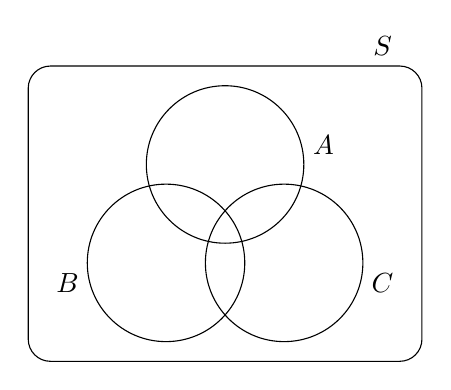
\begin{tikzpicture}[scale=0.5, every node/.style={scale=1}]
\draw [,rounded corners=8pt,] (0,0) -- (0,7.5) -- (10,7.5) -- (10,0) -- cycle;
\node  at (9,8) {$S$};
\draw (3.5,2.5) circle (2cm);
\node  at (1,2) {$B$};
\draw (6.5,2.5) circle (2cm);
\node  at (9,2) {$C$};
\draw (5,5) circle (2cm);
\node  at (7.5,5.5) {$A$};
\end{tikzpicture}

\end{minipage}
\begin{minipage}{0.35\textwidth}
\centering
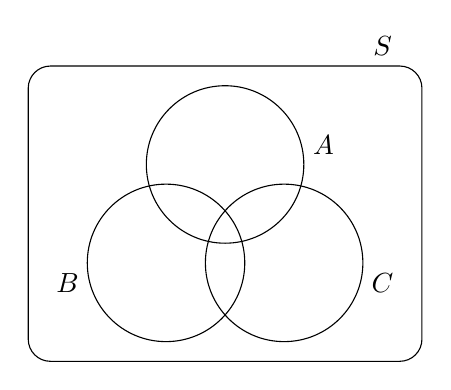
\begin{tikzpicture}[scale=0.5, every node/.style={scale=1}]

\draw [,rounded corners=8pt,] (0,0) -- (0,7.5) -- (10,7.5) -- (10,0) -- cycle;
\node at (9,8) {$S$};
\draw (3.5,2.5) circle (2cm);
\node at (1,2) {$B$};
\draw (6.5,2.5) circle (2cm);
\node at (9,2) {$C$};
\draw (5,5) circle (2cm);
\node at (7.5,5.5) {$A$};
\end{tikzpicture}

\end{minipage}
\caption{Diagramas de Venn com três conjuntos: \(A\), \(B\)  e \(C\)}
\label{diagramavenn3}
\end{figure}
\end{task}

\explore{regras básicas e propriedades}

No início do século XX, o matemático russo Kolmogorov, como já comentado na Seção \hyperref[conceitosbasicos]{Explorando: Probabilidade \textendash{} conceitos básicos}, estabeleceu regras básicas para a probabilidade que independem da interpretação adotada, possibilitando assim, a construção de uma teoria matemática de probabilidade.

De maneira simplificada, essas regras básicas serão apresentadas a seguir.

Seja \(S\) um espaço amostral. Uma probabilidade é uma função \(P\) que associa a cada subconjunto de \(S\) (evento)  um número real, tal que
\begin{enumerate}
\item {} 
ela é sempre um número não negativo,

\item {} 
a probabilidade do evento certo é igual a 1 e,

\item {} 
dados dois eventos disjuntos, a probabilidade da união dos dois é dada pela soma das probabilidades individuais.

\end{enumerate}

Em símbolos, essas regras podem ser apresentadas da seguinte forma:
\begin{enumerate}
\item {} 
\(P(A)\geq 0\) qualquer que seja \(A\subset S\), ou seja, a probabilidade de qualquer evento \(A\) é um número não-negativo.

\item {} 
\(P(S)=1\), ou seja, a probabilidade do evento certo é igual a 1.

\item {} 
Se \(A,B\subset S\) com \(A\) e \(B\) eventos disjuntos (\(A\cap B=\emptyset\)), então \(P(A\cup B)=P(A)+P(B)\).

\end{enumerate}
\begin{task}{censo Educação Física}


Em uma escola de Ensino Médio há dois turnos: manhã e tarde. No turno da manhã há 450 alunos e, no turno da tarde, 350 alunos. Os professores de Educação Física realizaram um censo para saber se os alunos da escola praticavam algum tipo de atividade física regular fora do período escolar. A pergunta principal do questionário da pesquisa foi:

\textbf{Qual é a sua atividade física principal fora do período escolar? Marque apenas uma opção.}


\begin{center}\textbf{(  ) Não pratica  (   ) Futebol (  ) Outra}\end{center}

Na \hyperref[frequenciaatividade]{tabela \ref{frequenciaatividade}} estão os resultados obtidos.
\begin{quote}

\end{quote}

\begin{table}[H]
\centering
\begin{tabu} to \textwidth{|c|c|c|c|}
\hline
\thead
Atividade Física & Manhã & Tarde & Total \\
\hline
Não pratica & 140 & 130 & 270 \\
\hline
Futebol & 160 & 80 & 240 \\
\hline
Natação & 80 & 70 & 150 \\
\hline
Outra atividade & 70 & 70 & 140 \\
\hline
Total & 450 & 350 & 800 \\
\hline
\end{tabu}
\caption{Distribuição de frequências por atividade, segundo o turno.}
\label{frequenciaatividade}
\end{table}

Um aluno desta escola será escolhido ao acaso.
\begin{enumerate}
\item {} 
Considere os eventos \(A\):  ” o aluno escolhido não pratica atividade física”, \(B\): ” o aluno escolhido pratica Futebol como atividade física principal”, \(C\): ” o aluno escolhido pratica natação” e \(D:\): “o aluno pratica outro tipo de atividade física principal”. Determine a probabilidade de cada um desses eventos.

\item {} 
Observe que o espaço amostral nesse experimento corresponde à união dos eventos considerados no item anterior. Calcule a soma das probabilidades determinadas no item anterior. O resultado obtido é compatível com a segunda regra básica, a saber, \(P(S)=1\)? Por quê?

\item {} 
Qual é a probabilidade de que este aluno pratique algum tipo de atividade física regular fora do período escolar?

\item {} 
O que é mais provável: que o aluno escolhido seja do turno da manhã e jogue futebol ou que o aluno jogue futebol?

\item {} 
Qual é a probabilidade de que o aluno escolhido seja do turno da tarde \textbf{ou} pratique atividade física diferente de futebol, isto é, que o aluno escolhido tenha pelos menos uma dessas duas características?

\end{enumerate}
\end{task}


\arrange{regras básicas e propriedades}

A última regra básica é chamada propriedade aditiva da probabilidade para eventos disjuntos e, de fato, é um caso particular da propriedade de aditividade da probabilidade.

Suponha três eventos \(A\), \(B\) e \(C\) disjuntos 2 a 2, ou seja, \(A\cap B=A\cap C=B\cap C=\emptyset\). A regra da aditividade para a união destes três eventos resultará em \(P(A\cup B\cup C)=P(A)+P(B)+P(C)\).
\begin{figure}[H]
\centering

\begin{tikzpicture}[scale=0.8]

\draw [,rounded corners=8pt, -] (0,0) -- (0,8) -- (10,8) -- (10,0) -- cycle;
\node at (9,8.25) {$S$};
\draw [fill=\currentcolor!80](2.5,2.2) circle (2cm);
\node  at (.75,.5) {$B$};
\draw [fill=\currentcolor!80](7.5,2.2) circle (2cm);
\node  at (9.25,.5) {$C$};
\draw [fill=\currentcolor!80](5,5.75) circle (2cm);
\node  at (7.5,5.5) {$A$};
\end{tikzpicture}

\caption{Três eventos A, B e C disjuntos dois a dois ilustrados no diagrama de Venn}

\end{figure}

A propriedade de aditividade da probabilidade para eventos disjuntos vale para qualquer coleção de eventos disjuntos 2 a 2.


\subsection{Interpretações da probabilidade e as regras básicas}

Como determinar probabilidades sob cada uma das interpretações apresentadas na Seção \hyperref[organizandoconceitosbasicos]{Organizando as ideias: Probabilidade \textendash{} conceitos básicos}, considerando as regras básicas?

\textbf{1. Interpretação clássica}

\begin{example}{}

Considere o lançamento de um dado honesto (todas as faces ocorrem com probabilidades iguais). Neste caso o espaço amostral é dado por

\(S=\{ 1,2,3,4,5,6\}\) e, os eventos elementares, são dados por

$$A_1=\{1\}, A_2=\{2\}, A_3=\{3\}, A_4=\{4\}, A_5=\{5\} \text{ e } A_6=\{6\}.$$

Faça \(P(A_i)=k\), \(i=1,2,3,4,5,6\).

Observe que \(S=A_1\cup A_2\cup A_3\cup A_4\cup A_5 \cup A_6\) e que os eventos \(A_1\), \(A_2\), \(A_3\), \(A_4\) , \(A_5\) e \(A_6\) são disjuntos.

Usando as regras básicas, tem-se

$$1=P(S)=P(A_1\cup A_2\cup A_3\cup A_4\cup A_5 \cup A_6)=P(A_1)+P(A_2)+\cdots +P(A_6)=6\cdot k$$

Logo, \(k=\frac{1}{6}\).
\end{example}

De modo mais geral, sob a interpretação clássica na qual o espaço amostral \(S\) é finito e todos os eventos elementares são equiprováveis, se o número de elementos do conjunto \(S\) é \(n\), \(n\in \mathbb{N}\), então a probabilidade de um evento elementar é dada por \(\frac{1}{n}\).

Nesse caso, se \(A\subset S\) tem-se $\displaystyle{P(A)=\frac{\#(A)}{n}}$, em que a notação \(\#(A)\) representa o número de elementos do conjunto \(A\).

\begin{observation}{ }

\textbf{Observação} Usando a interpretação clássica, na qual o espaço amostral \(S\) é um conjunto finito e todos os eventos elementares são equiprováveis, tem-se que \(P(A)=\frac{\#(A)}{\#(S)}\).

Observe que as regras básicas são satisfeitas, pois
\begin{enumerate}
\item {} 
\(P(A)=\displaystyle{\frac{\#(A)}{\#(S)}}\geq 0\), qualquer que seja \(A \subset S\);

\item {} 
\(P(S)=\displaystyle{\frac{\#(S)}{\#(S)}=1}\) e,

\item {} 
se \(A\cap B=\emptyset\), tem-se que \(\#(A\cup B)=\#(A)+\#(B)\) tal que \(P(A\cup B)=P(A)+P(B)\).

\end{enumerate}

\textbf{Atenção:} Antes de sair usando essa interpretação, é necessário verificar se a suposição de eventos elementares equiprováveis é adequada. Por exemplo, vimos no item b) da Atividade \emph{o espaço amostral não é único}, que \(S=\{0,1,2,3\}\) com quatro elementos. No entanto, esses elementos não são igualmente prováveis, pois os eventos elementares \(\{1\}\) e \(\{ 2\}\) são três vezes mais prováveis de ocorrer comparados aos eventos elementares \(\{0\}\) e \(\{3\}\).
\end{observation}

\textbf{2. Interpretação frequentista}

Na interpretação frequentista atribuem-se probabilidades, usando-se as frequências relativas de ocorrência do evento depois de observar o mesmo experimento um grande número de vezes. Também podemos perceber com esta interpretação, que as regras da probabilidade valem, pois uma frequência relativa é sempre um número não-negativo. Se considerarmos o evento certo, é claro que sua frequência relativa de ocorrência será sempre 1, independente até da quantidade de vezes na qual o experimento é repetido. Finalmente, dados dois eventos disjuntos, a frequência relativa de ocorrência da união dos dois será dada pela soma das frequências relativas dos dois.

\textbf{3. Interpretação subjetiva}

A validade das regras básicas na interpretação subjetiva de probabilidade depende de coerência com as regras básicas, quando se atribuem probabilidades. Por exemplo, para um espaço amostral \(S\) finito, as probabilidades atribuídas aos eventos elementares não devem ser valores fora do intervalo \([0,1]\). Além disso, a soma das probabilidades dos eventos elementares deverá ser igual a 1.


\subsection{Propriedades da probabilidade}

A seguir, serão enumeradas algumas propriedades úteis no cálculo de probabilidades. Estas propriedades são consequências das regras básicas da probabilidade.

\begin{description}
\item[Propriedade 1] A probabilidade do evento vazio (\(\emptyset\)) é zero.
\end{description}

Esta propriedade é obtida das regras básicas \(P(S)=1\) e aditividade da probabilidade para eventos disjuntos, lembrando que \(S\cup \emptyset =S\) e \(S\cap \emptyset =\emptyset\).

Observe que de fato é natural que a probabilidade do evento vazio seja zero, pois um evento vazio nunca irá ocorrer.

\begin{description}
\item[Propriedade 2] A probabilidade de um evento \(A\) pode ser calculada por \(P({A})= 1-P(\overline{A})\).
\end{description}

Muitas vezes pode ser complicado calcular diretamente a probabilidade de um evento. Uma possível simplificação será calcular a probabilidade do evento complementar. Um exemplo comum, é o problema dos aniversários que será apresentado na seção \hyperref[regrasbasicaspropriedades]{Praticando: Probabilidade - regras básicas e propriedades}. Uma aplicação desta propriedade está ilustrada no item (c) da atividade \emph{censo Educação Física}.

\begin{description}
\item[Propriedade 3] Dados \(A\) e \(B\) eventos em um espaço amostral \(S`tais que `A\subset B\) (\(A\) está contido em \(B\)), então \(P(A)\leq P(B)\).
\end{description}

Essa propriedade, ilustrada no item d) da atividade \emph{censo Educação Física}, pode ser obtida a partir das regras básicas:
como \(A\subset B\), podemos escrever o evento \(B\) como a união de dois eventos disjuntos, a saber,  \(B=A\cup (B\cap \overline{A})\). Veja uma ilustração na \hyperref[eventosdijuntos]{figura \ref{eventosdijuntos}}.
\begin{figure}[H]
\centering

\begin{tikzpicture}

\draw [,rounded corners=8pt, -] (0,0) -- (0,7) -- (7,7) -- (7,0) -- cycle;
\node  at (6,7.3) {$S$};
\draw [fill=\currentcolor!80](3.5,3.5) circle (3cm);
\draw [fill=destacado!70] (5,3.5) circle (1cm);
\node [above right] at (1,6) {$B$};
\node at (5,3.5) {$A$};
\node at (3,2) {$\overline{A}\cap B$};
\end{tikzpicture}
\caption{\(B=A\cup (\overline{A}\cap B)\) como a união de dois eventos disjuntos}
\label{eventosdijuntos}
\end{figure}


Assim, usando a regra de que toda probabilidade é um número não-negativo e a regra básica de aditividade da probabilidade, tem-se
\begin{equation*}
\begin{split}P(B)=P(A\cup(\overline{A}\cap B))=P(A)+\underbrace{P(\overline{A}\cap B)}_{\geq 0}\geq P(A)\end{split}
\end{equation*}
\textbf{Propriedade 4} \(P(A\cup B)=P(A)+P(B)-P(A\cap B)\), quaisquer que sejam os eventos \(A\) e \(B\) de um espaço amostral \(S\).

Essa propriedade, utilizada no item (e) da Atividade \emph{censo Educação Física}, pode ser obtida, escrevendo-se o evento \(A\cup B\) como a união de dois eventos disjuntos, a saber, \(A\cup B=A\cup (\overline{A}\cap B)\).

Veja uma ilustração na \hyperref[eventosdijuntos2]{figura \ref{eventosdijuntos2}}.
\begin{figure}[H]
\centering

\begin{tikzpicture}
\node at (7,5.3) {$S$};
\draw [=,rounded corners=8pt, -] (0,-0) -- (0,5) -- (8,5) -- (8,0) -- cycle;
\node at (7,4) {$B$};
\node at (.5,4) {$A$};
\node at (4,-.5) {$A \cup B$};
\draw [fill=\currentcolor!80] (5,2.5) circle (2cm);
\node at (5.5 ,2) {$\overline{A}  \cap B$};
\draw [fill=\currentcolor!80] (2.5,2.5) circle (2cm) ;
\clip[draw] (5,2.5) circle (2cm);
\end{tikzpicture}

\caption{\(A\cup B\) como uma união de dois eventos disjuntos: \(A\cup (\overline{A}\cap B)\)}
\label{eventosdijuntos2}
\end{figure}

Assim, \(P(A\cup B)=P(A)+P(\overline{A}\cap B)\) , pois \(A\) e \(\overline{A}\cap B\) são disjuntos.

Mas, como \(B=(A\cap B) \cup (\overline{A}\cap B)\) e os eventos \(A\cap B\) e \(\overline{A}\cap B\) são disjuntos, segue que \(P(B)=P(A\cap B)+P(\overline{A}\cap B)\) (Veja a \hyperref[eventosdijuntos3]{figura \ref{eventosdijuntos3}}).

\begin{figure}[H]
\centering

\begin{tikzpicture}

\node at (7,5.3) {$S$};
\draw [ ,rounded corners=8pt, -] (0,-0) -- (0,5) -- (8,5) -- (8,0) -- cycle;
\node at (6.5,4) {$B$};
\node at (1,4) {$A$};
\draw [fill= \currentcolor!80] (4.5,2.5) circle (2cm);
\node at (5.75,2.5) {$\overline{A}  \cap B$};
\clip [draw]  (3,2.5) circle (2cm) ;
\draw [fill= \currentcolor!40] (4.5,2.5) circle (2cm);
\node at (3.75,2.5) {$A\cap B$};
\end{tikzpicture}
\caption{\(B\) como a união de dois eventos disjuntos.}
\label{eventosdijuntos3}
\end{figure}

Logo, podemos escrever \(P(\overline{A}\cap B)=P(B)-P(A\cap B)\) tal que
\begin{equation*}
\begin{split}P(A\cup B)=P(A)+P(B)-P(A\cap B)\end{split}
\end{equation*}


\practice{regras básicas e propriedades}
\label{regrasbasicaspropriedades}\begin{task}{o problema dos bodes}


Em um programa de televisão semanal, um jogo oferece como prêmio um automóvel a um espectador escolhido da plateia. O candidato a ganhar o automóvel é convidado pelo apresentador do programa a escolher uma entre três portas idênticas, atrás das quais há um carro em uma delas e, nas outras duas, há um bode em cada uma.

\begin{figure}[H]
\centering

\noindent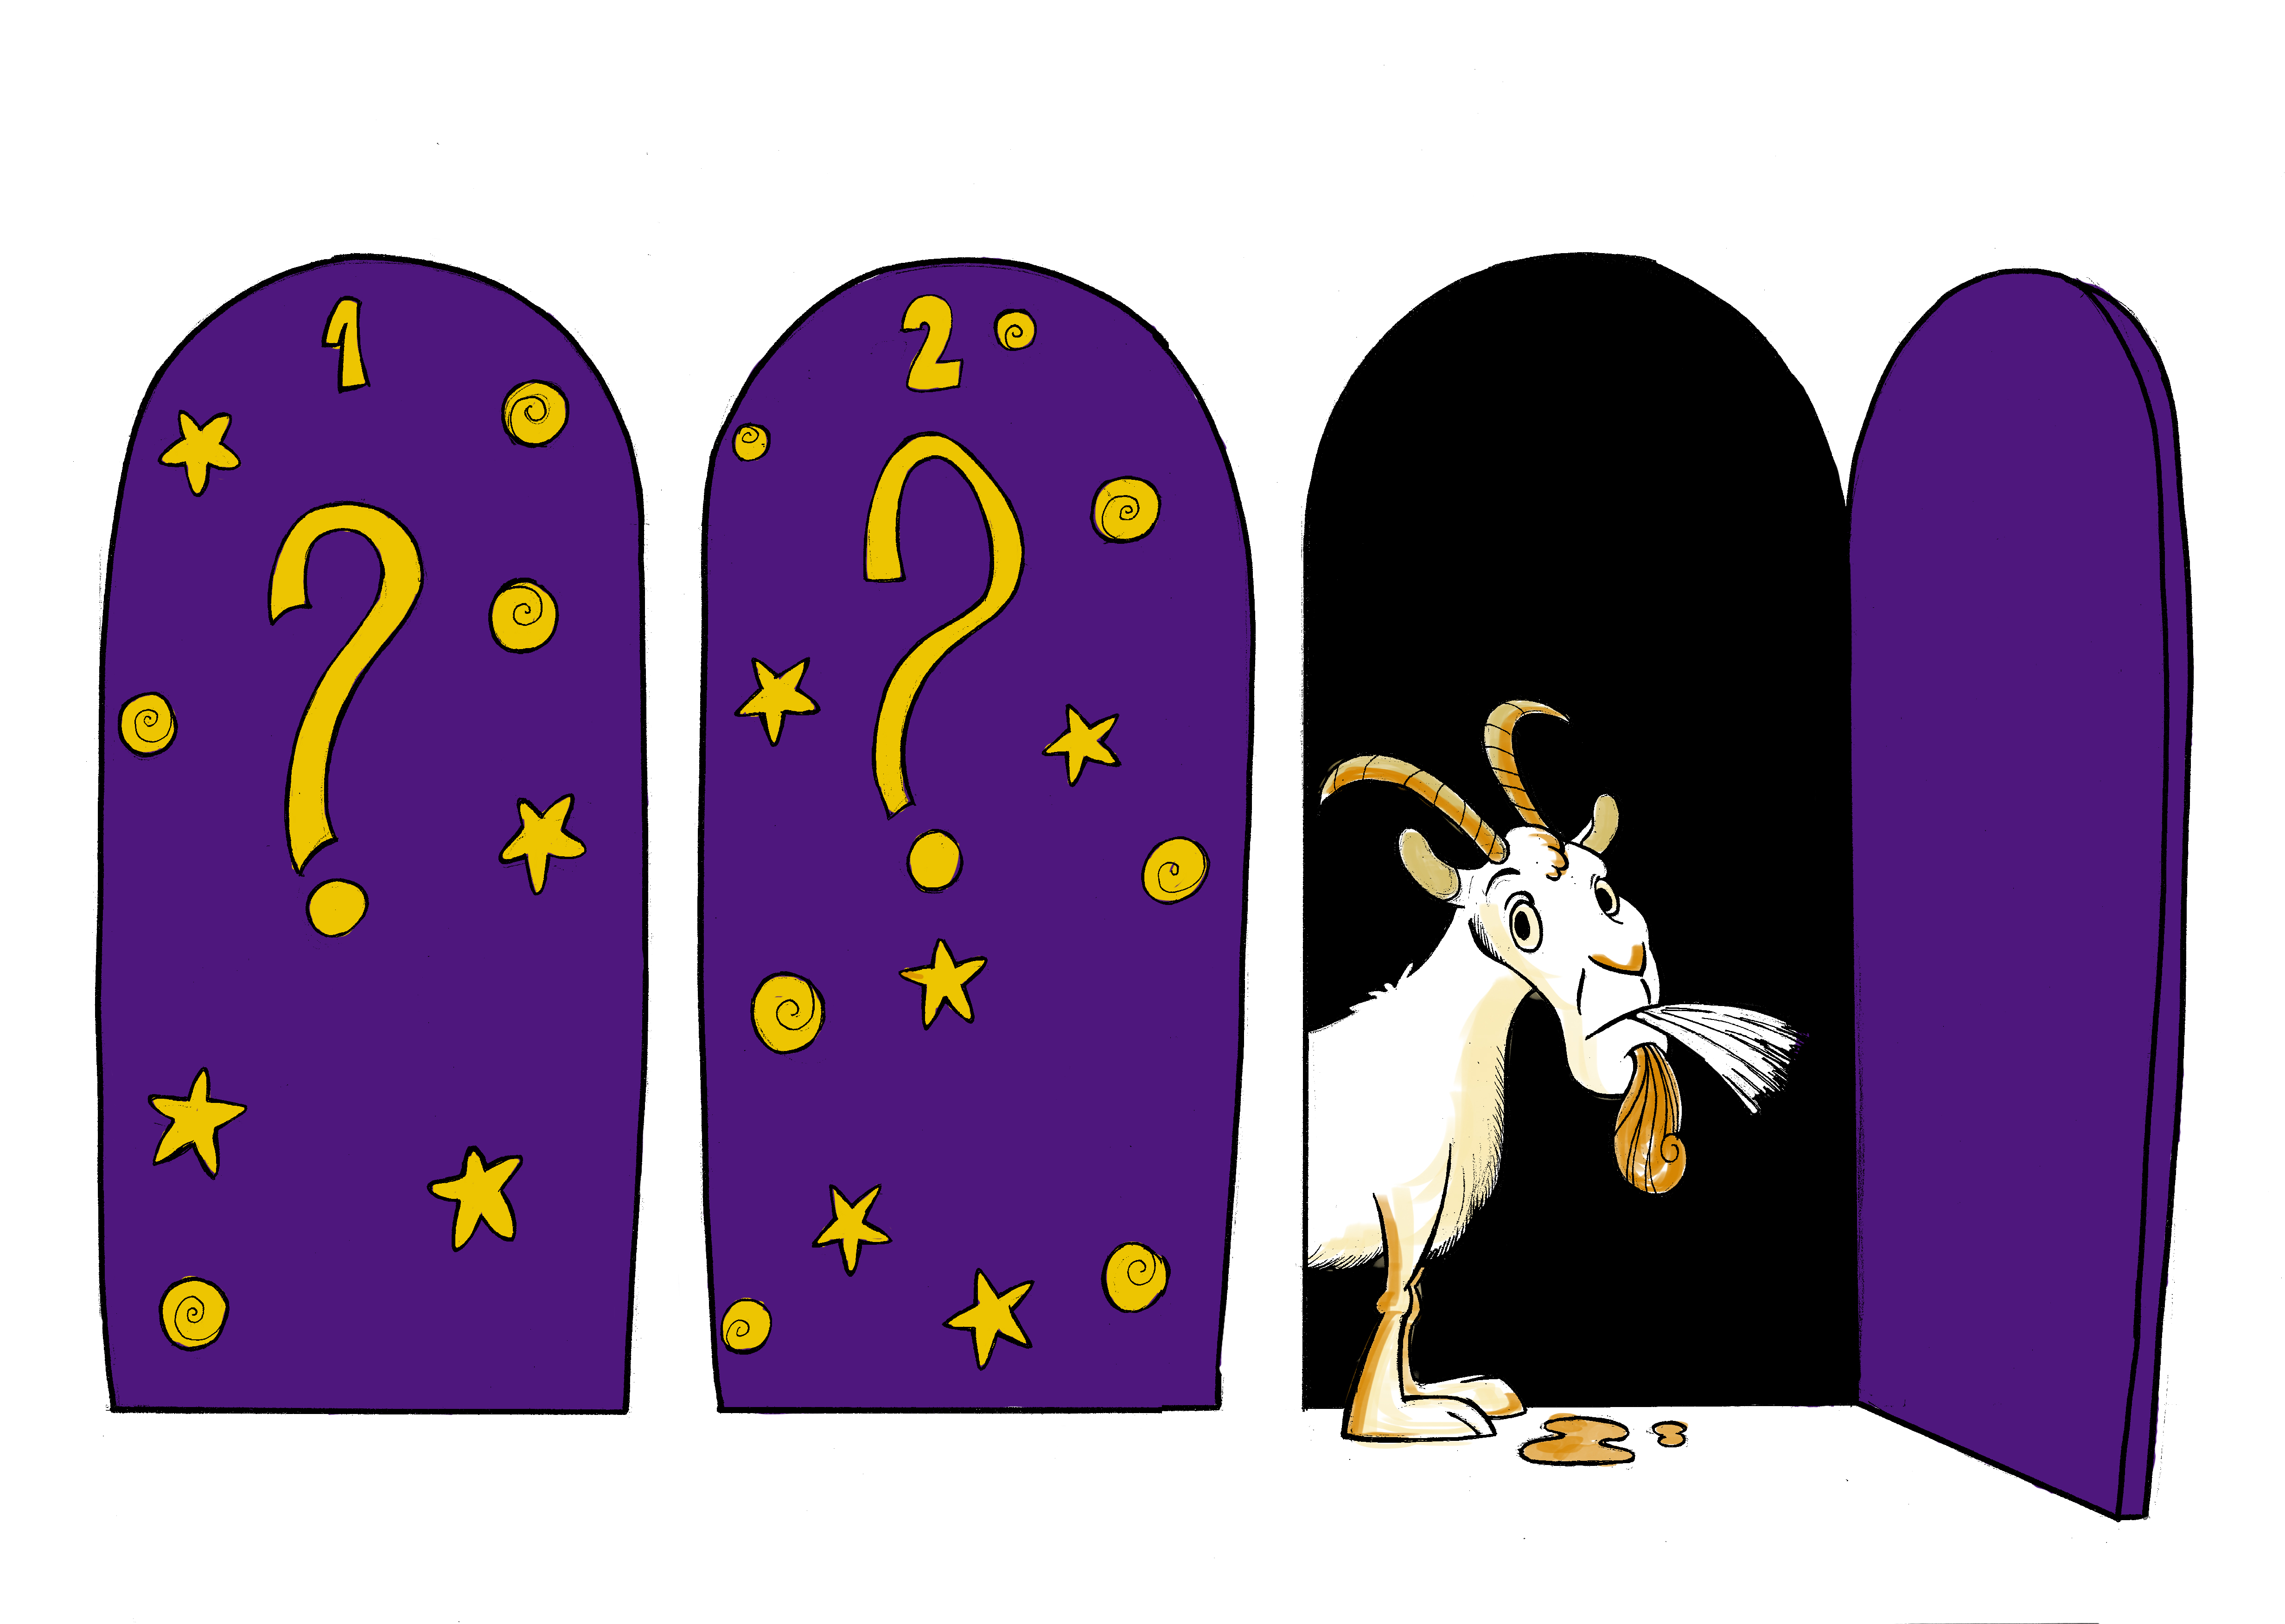
\includegraphics[width=250bp]{bode}
\caption{Problema dos bodes}
\end{figure}


Depois de o candidato escolher a porta, o apresentador, que sabe o que tem atrás de cada uma delas, abre uma das portas não escolhidas, mostrando que atrás dela tem um bode. Então, o apresentador oferece ao candidato decidir entre manter sua escolha inicial ou trocar de porta.

Qual deve ser a melhor estratégia para o candidato (trocar ou não trocar de porta) de modo que a sua probabilidade de ganhar o automóvel seja a maior possível?
\end{task}
\begin{task}{jogo de dardos}



No jogo de dardos o vencedor é quem zera os seus pontos mais rapidamente. Você começa, por exemplo, com um total de 200 pontos. A cada lançamento do dardo, dependendo do local atingido, você ganha uma certa pontuação que é descontada do seu total. Se você for o primeiro a zerar, será o vencedor do jogo.

Quanto mais próximo do centro do tabuleiro de dardos (um tabuleiro circular conforme a \hyperref[dardos]{figura \ref{dardos}}), mais pontos você ganha.

Suponha que você seja suficentemente experiente de modo que todos os seus lançamentos atingem o tabuleiro de dardos.

\begin{figure}[H]
\centering


\begin{tikzpicture}[scale=1.5]

\draw [fill= secundario!70] (0,0) circle (2);
\draw [fill= white!70] (0,0) circle (1.85);
\draw [fill= \currentcolor!70] (0,0) circle (1.55);
\draw [fill= white!70] (0,0) circle (1);
\draw [fill= \currentcolor!70] (0,0) circle (.5);
\draw [fill= destacado!70] (0,0) circle (.1);
\draw [fill=secundario] (1.4142,1.4142) arc (45:-135:2);
\draw [fill=secundario!7] (1.30814,1.30814) arc (45:-135:1.85);
\draw [fill=\currentcolor] (1.0960,1.0960) arc (45:-135:1.55);
\draw [fill=secundario!7] (.70710,.70710) arc (45:-135:1);
\draw [fill=\currentcolor] (.35355,.35355) arc (45:-135:.5);
\draw [fill=destacado] (.070710,.070710) arc (45:-135:.1);
\draw [,color=blue!30!\currentcolor, fill=blue!30!\currentcolor] (1.8,1.8)--++(15:.2) --(2.19318,2.05176) -- (2,2);
\draw [,color=blue!30!\currentcolor, fill=blue!30!\currentcolor] (1.8,1.8)--++(75:.2) --(2.05176,2.19318) --(2,2);
\draw [] (0,0) -- (2.04,2.04);
\draw [secundario!7] (-1.29814,-1.29814)--(-1.1060,-1.1060);
\draw [secundario!7] (-.69710,-.69710)--(-.36355,-.36355);
\draw [destacado] (-.066710,-.066710)--(0,0);
\end{tikzpicture}
\caption{Tabuleiro de jogo de dardos}
\label{dardos}
\end{figure}

Suponha que a medida do raio do tabuleiro de dardos seja 20 cm e que a medida do menor raio (círculo em verde no centro do tabuleiro) seja 5 cm, e que os acréscimos de comprimento do raio nas faixas branca, verde e branca do tabuleiro sejam iguais a 5 cm. A moldura em preto não faz parte do alvo. Suponha também que atingindo o
\begin{enumerate}
\item {} 
círculo de raio 5 cm (em verde), você ganha 100 pontos;

\item {} 
o anel cicular mais próximo ao centro (em branco), você ganha 50 pontos;

\item {} 
o anel circular em verde subsequente, você ganha 20 pontos e

\item {} 
a anel circular mais externo (em branco), você ganha 10 pontos.

\end{enumerate}


Observe que, neste caso, não é possível usar a interpretação clássica de probabilidade, pois existem infinitos eventos elementares. No entanto, é razoável supor uniformidade de probabilidades se, de fato, o jogador acerte em qualquer ponto do tabuleiro de dardos ao acaso.  Neste espaço amostral, o círculo de raio 20 cm, se os pontos são obtidos ao acaso, ao considerar regiões de mesma área, contidas no círculo, as probabilidades de se obter pontos nestas regiões devem ser iguais.

Assim, calcula-se a probabilidade do dardo cair numa região dentro do círculo como o quociente entre a medida da área da região sobre a medida da área do círculo (espaço amostral), isto é, se
\begin{equation*}
\begin{split}A\subset S \textsf{, então } P(A)=\displaystyle{\frac{\textsf{Área de }A}{\textsf{Área de }S}}\end{split}
\end{equation*}

\begin{figure}[H]
\centering

\begin{tikzpicture}[scale=0.75]  

\draw [thick] (0,0) circle (5cm);
\draw [fill = \currentcolor!50, thick]  (1.5,1.5) circle (2cm);
\node at (2,2) {$A$};

\node at (2.5,5) {$S$};
\end{tikzpicture}


\caption{Exemplo de um evento \(A\) no tabuleiro de dardos}
\end{figure}

Observações:
\begin{enumerate}
\item {} 
Nesta situação, a probabilidade do dardo atingir um ponto fixado no círculo será sempre zero, pois a medida de área correspondente a um ponto é nula.

\item {} 
Esta forma de calcular probabilidades costuma ser denominada como \emph{probabilidade geométrica} e pode ser considerada como uma extensão da interpretação clássica de probabilidade para espaços amostrais representados por uma região do plano com área definida. Esta mesma noção poderá ser usada para espaços amostrais representados por intervalos da reta limitados de comprimento definido, neste caso, calculando-se probabilidades como uma razão de comprimentos de intervalos.

\end{enumerate}

Calcule a probabilidade de que em um lançamento você ganhe
\begin{enumerate}
\item {} 
exatamente 100 pontos;

\item {} 
exatamente 20 pontos;

\item {} 
no máximo 50 pontos.

\item {} 
Suponha também que pode ser combinado, antes do início do jogo, conceder um bônus adicional de 10\% da pontuação, se o dardo atingir o semicírculo, destacado na \hyperref[dardos]{figura \ref{dardos}}. Calcule a probabilidade de que em um lançamento você atinja
\begin{enumerate}
\item {} 
o semicírculo destacado ou uma faixa de exatamente 50 pontos;

\item {} 
o semicírculo destacado e uma faixa de pelo menos 20 pontos.

\end{enumerate}

\end{enumerate}
\end{task}

\begin{task}{o problema dos aniversários}


Numa turma de seu colégio há 35 alunos. Calcule a probabilidade de que haja pelo menos uma coincidência de datas de aniversário (dia e mês) entre os alunos dessa turma. Considere apenas anos não bissextos e suponha que todos os 365 dias do ano são igualmente prováveis como datas de aniversário.

\begin{figure}[H]
\centering

\noindent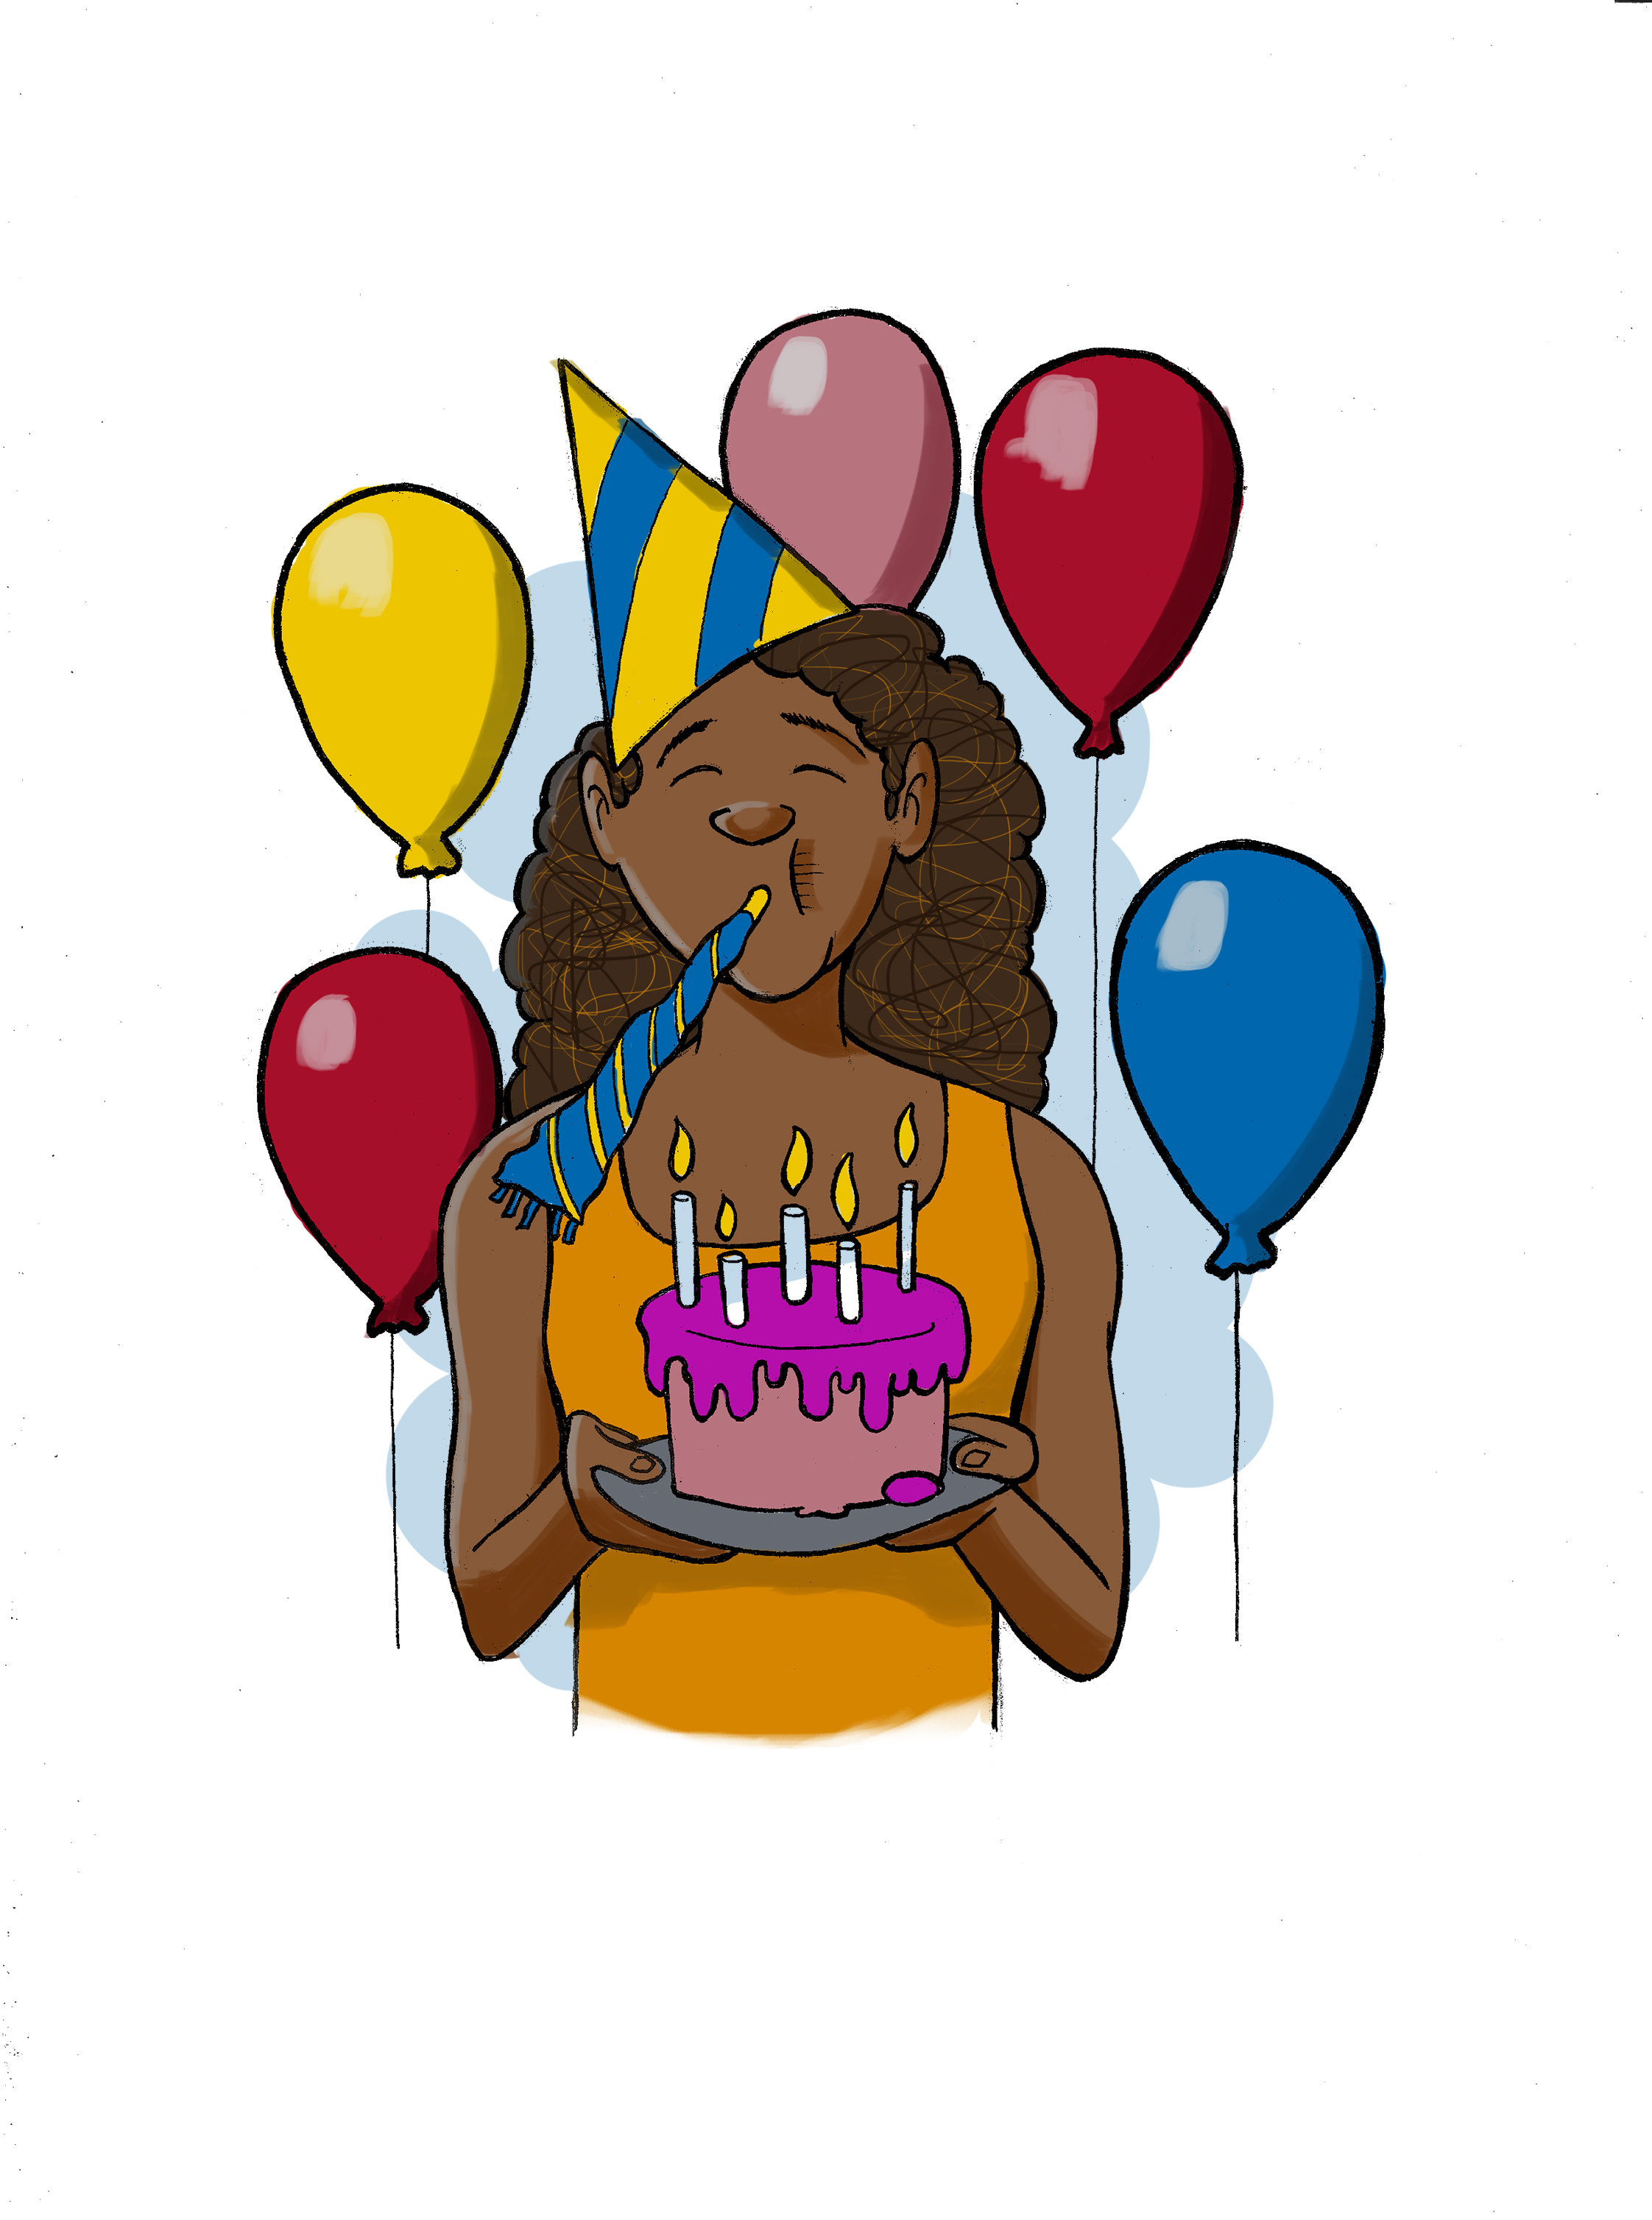
\includegraphics[width=200bp]{bolo.jpg}
\end{figure}
\end{task}


\explore{ Probabilidade Condicional}


\begin{task}{uso de óculos e sexo de estudandes}


Na tabela a seguir estão os dados de uma turma de segundo ano do Ensino Médio com 40 alunos quanto ao gênero e se ele usa ou não óculos.

\begin{table}[H]
\centering
\begin{tabu} to \textwidth{|l|c|c|c|}
\hline
\thead
gênero & usa óculos & não usa óculos & total \\
\hline
feminino & 6 & 16 & 22 \\ 
\hline
masculino & 5 & 13 & 18 \\
\hline
total & 11 & 29 & 40 \\
\hline
\end{tabu}
\end{table}

Se um estudante desta turma é sorteado, pede-se determinar a probabilidade de que ele
\begin{enumerate}
\item {} 
use óculos;

\item {} 
use óculos, sabendo que é do gênero feminino;

\item {} 
use óculos, sabendo que é do gênero masculino;

\item {} 
seja do gênero feminino;

\item {} 
seja do gênero feminino, sabendo que usa óculos;

\item {} 
seja do gênero feminino, sabendo que não usa óculos.

\item {} 
Analisando os dados da tabela e as respostas obtidas, há razões para supor que gênero é independente de uso de óculos ou não? Por quê?

\end{enumerate}
\end{task}


\arrange{ Probabilidade Condicional}


\subsection{Definição de probabilidade condicional}

Em Ciência,  “informação disponível”  é certamente uma matéria-prima preciosa, pois através dela é possível construir modelos mais realísticos para descrever  fenômenos tanto determinísticos quanto aleatórios e obter resultados mais fidedignos de um ponto de vista da aplicação. Assim, quanto mais informação dispomos sobre determinados fenômenos, mais acurados serão potencialmente nossos modelos. É nesse sentido que surge historicamente o conceito de probabilidade condicional, tema dessa seção.

A ideia central da probabilidade condicional é estabelecer uma estrutura matemática para reavaliar a probabilidade de um evento à luz de uma informação disponível relacionada a este. Por exemplo, um geólogo, ao examinar uma bacia, avaliará a probabilidade de potencial petrolífero de forma diferente a depender de informações disponíveis, tais como porosidade da rocha, estruturas sísmicas, etc. Quanto mais informação ele tenha, tanto mais próxima da realidade será potencialmente sua avaliação da probabilidade de encontrar óleo na região.

\begin{figure}[H]
\centering

\noindent\includegraphics[width=200bp]{{bacia_petroleo}.png}

\caption{Bacias de petróleo na costa brasileira}
\end{figure}



O mesmo se dá em avaliações médicas: a partir da anamnese do paciente, um médico melhorará sua avaliação sobre a probabilidade de um paciente ter ou não determinada patologia.

\begin{figure}[H]
\centering

\noindent\includegraphics[width=200bp]{{anamnese}.png}

\caption{Medição da pressão arterial para anamnese do paciente}
\end{figure}


A questão que se coloca é: como incorporar matematicamente a informação de que um evento B ocorreu para se reavaliar a ocorrência de um evento de interesse A?

A definição de probabilidade condicional é a resposta para essa questão.

\begin{description}
\item[Definição]

A probabibilidade condicional de o evento \(A\) ocorrer, dado que sabemos que o evento \(B\)  ocorreu, denotada por \(P(A|B)\),  é definida por
\begin{equation*}
\begin{split}P(A|B)=\frac{P(A\cap B)}{P(B)}, \quad P(B)>0\end{split}
\end{equation*}\end{description}

Retomando a a Atividade \emph{uso de óculos e sexo de estudantes}, a probabilidade de o aluno sorteado usar óculos, sabendo que ele é do gênero masculino foi calculada pela razão do número de estudantes que usam óculos e são do gênero masculino e o número de estudantes do gênero masculino, a saber, \(\frac{5}{18}\approx 0,278\).

Observe que esse quociente, pode ser também obtido a partir da definição de probabilidade condicional, calculando-se o quociente da probabilidade de “usar óculos e ser do gênero masculino” (5/40=0,125) e da probabilidade de ser do gênero masculino (18/40=0,45), obtendo-se \(\displaystyle{\frac{0,125}{0,45}=\frac{5}{18}\approx 0,278}\).

Repita essa verificação para as demais probabilidades condicionais calculadas na Atividade \emph{uso de óculos e sexo de estudantes}.

\begin{example} {A probabilidade condicional é uma probabilidade?}

É possível verificar que a probabilidade condicional, \textbf{dado o conhecimento da ocorrência do evento B}, satisfaz as regras básicas da probabilidade e, portanto, também satisfaz as demais propriedades da probabilidade trabalhadas na seção anterior.

A primeira regra básica é a de que toda probabilidade é um número não negativo. De fato, tem-se que dado um evento \(A\subset S\) qualquer,
\begin{equation*}
\begin{split}P(A|B)=\frac{\overbrace{P(A\cap B)}^{\geq 0}}{\underbrace{P(B)}_{>0}}\geq 0\end{split}
\end{equation*}
Além disso, a segunda propriedade básica \(P(S)=1\) pode ser adaptada.  Observe que dado que o evento \(B\) ocorreu, o natural é passar a considerá-lo como o “novo” espaço amostral à luz dessa informação. Assim,
\begin{equation*}
\begin{split}P(B|B)=\frac{P(B)}{P(B)}=1\end{split}
\end{equation*}
de modo que vale a segunda regra básica.

Finalmente, dados \(A_1\) e \(A_2\)  eventos disjuntos,
\begin{equation*}
\begin{split}P(A_1\cup A_2|B)=\frac{P(A_1\cup A_2)\cap B)}{P(B)}=\frac{P((A_1\cap B)\cup(A_2\cap B))}{P(B)}\end{split}
\end{equation*}
Na expressão anterior, observe que foi usada a propriedade distributiva da operação de interseção com a união de dois eventos. Observe também que, no numerador do termo mais à direita da expressão obtida, tem-se a probabilidade da união de dois eventos, a saber, \(A_1\cap B\) e \(A_2\cap B\).

Como os eventos \(A_1\) e \(A_2\) são disjuntos, consequentemente, os eventos \(A_1\cap B\subset A_1\) e \(A_2\cap B\subset A_2\)  também são disjuntos tal que \(P((A_1\cap B)\cup(A_2\cap B))=P(A_1\cap B)+P(A_2\cap B)\) (regra básica 3 da probabilidade).

Logo,
\begin{equation*}
\begin{split}P(A_1\cup A_2|B)=\frac{P((A_1\cup A_2)\cap B)}{P(B)}=\frac{P(A_1\cap B)+P(A_2\cap B)}{P(B)}=P(A_1|B)+P(A_2|B)\end{split}
\end{equation*}
Portanto, as demais propriedades da probabilidade estudadas, também valem para a probabilidade condicional, a saber,
\begin{enumerate}
\item {} 
\(P(\emptyset |B)=0\)

\item {} 
Se \(A_1\subset A_2\),  então \(P(A_1|B)\leq P(A_2|B)\).

\item {} 
\(P(A|B)=1-P(\overline{A}|B)\).

\item {} 
\(P(A_1 \cup A_2|B)=P(A_1|B)+P(A_2|B)-P(A_1\cap A_2|B)\).

\end{enumerate}
\end{example}


\subsection{Regra da Multiplicação}

A partir da definição de probabilidade condicional é possível obter uma regra para calcular a probabilidade da ocorrência simultânea de dois eventos \(A\)  e \(B\). Como \(\displaystyle{P(A|B)=\frac{P(A\cap B)}{P(B)}}\), segue que
\begin{quote}
\begin{equation*}
\begin{split}P(A\cap B)=P(B)\cdot P(A|B)\end{split}
\end{equation*}\end{quote}

Essa expressão é fundamental para entender resoluções de problemas de cálculo de probabilidades em experimentos sequenciais. Veja o exemplo a seguir.

\begin{example} {Diagrama de árvore}

Em um grupo de 12 pessoas, sabe-se que 8 delas votarão no candidato à prefeito  \(ABC\) e as outras 4 votarão no candidato a prefeito \(XYZ\). Suponha que duas pessoas serão escolhidas sequencialmente, ao acaso e sem reposição desse grupo. Deseja-se calcular a probabilidade de que as duas pessoas sorteadas votarão em candidatos a prefeito distintos.

Primeiro vamos apresentar uma solução analítica desse problema, para em seguida mostrar a solução, muito mais simples, usando diagrama de árvore. A solução analítica será útil para compreender melhor os elementos da árvore e quando usar multiplicação e adição de probabilidades.

Como são apenas dois candidatos, vamos chamar de \(A_1\) o evento “a primeira pessoa sorteada votará em \(ABC\) ” e, assim, \(\overline{A_1}\) corresponderá ao evento “a primeira pessoa sorteada votará em \(XYZ\) “. Similarmente, vamos chamar de \(A_2\) o evento “a segunda pessoa sorteada votará em \(ABC\) ” e, assim, \(\overline{A_2}\) corresponderá ao evento “a segunda pessoa sorteada votará em \(XYZ\) “. O evento cuja probabilidade queremos calcular é \(E\): “as duas pessoas sorteadas votarão em candidatos distintos.”

Observe que \(E=(A_1\cap \overline{A_2})\cup (\overline{A_1}\cap A_2)\)  e que os dois eventos do lado direito são disjuntos de modo que podemos calcular \(P(E)\) como a soma \(P(A_2\cap \overline{A_1})+P(\overline{A_2}\cap A_1)\). Observe que cada uma dessas duas probabilidades envolve a ocorrência simultânea de dois eventos, de modo que podemos usar a regra da multiplicação:

$$P(A_1\cap \overline{A_2})=P({A_1})\cdot \underbrace{P(\overline{A_2}|{A_1})}_{\mathclap{\substack{\textsf{prob. da 2a. pessoa não votar em ABC,} \\ \textsf{dado que a primeira vota em ABC}}}}=\frac{8}{12}\cdot\frac{4}{11}=\frac{8}{33}$$

$$P(\overline{A_1}\cap {A_2})=P(\overline{A_1})\cdot \underbrace{P({A_2}|\overline{A_1})}_{\mathclap{\substack{\textsf{prob. da 2a. pessoa votar em ABC,} \\ \textsf{dado que a primeira não vota em ABC}}}}=\frac{4}{12}\cdot\frac{8}{11}=\frac{8}{33}$$

Logo, \(\displaystyle{P(E)=\frac{8}{33}+\frac{8}{33}=\frac{16}{33}\approx 0,485}\)

\textbf{Solução via diagrama de árvore:} Cada ponto de ramificação da árvore  desdobra-se nas possibilidades. Observe que nesse exemplo há apenas duas, de modo que do primeiro ponto partem duas possibilidades e a partir de cada possibilidade, partirão mais duas possibilidades, como no esquema a seguir.
\begin{figure}[H]
\centering

\begin{tikzpicture}

\draw (0,0) -- (30:3) node [right] {$A_1$} node [above, midway, rotate=30, scale=0.7] {};
\draw (0,0) -- (-30:3) node [right] {$\overline{A_1}$} node [below, midway, rotate=-30, scale=0.7] {};
\draw (3.159807,1.5) -- ++(20:3) node [right] {$A_2$} node [above, midway, rotate=20, scale=0.7] {};
\draw (3.159807,1.5) -- ++(-20:3) node [right] {$\overline{A_2}$} node [below, midway, rotate=-20, scale=0.7] {};
\draw (3.159807,-1.5) -- ++(20:3) node [right] {$A_2$} node [above, midway, rotate=20, scale=0.7] {};
\draw (3.159807,-1.5) -- ++(-20:3) node [right] {$\overline{A_2}$} node [below, midway, rotate=-20, scale=0.7] {};
\end{tikzpicture}
\caption{Ilustração das quatro configurações possíveis via diagrama de árvore}
\end{figure}

Em cada ramificação, assinalamos a respectiva probabilidade. Veja na \hyperref[arvore2]{figura \ref{arvore2}}, o diagrama de árvore com as respectivas probabilidades destacadas.

\begin{figure}[H]
\centering


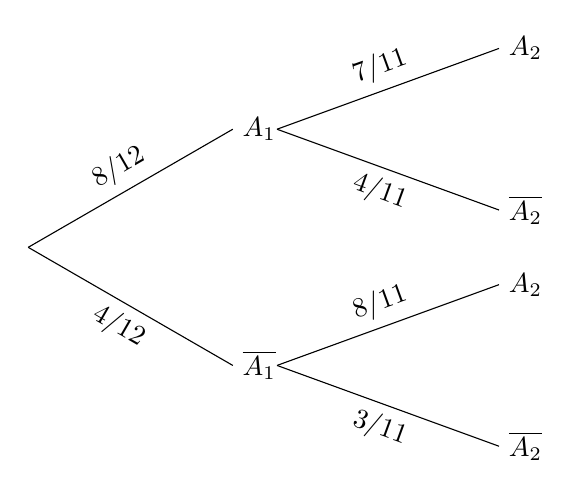
\begin{tikzpicture}

\draw (0,0) -- (30:3) node [right] {$A_1$} node [above, midway, rotate=30] {$8/12$};
\draw (0,0) -- (-30:3) node [right, ] {$\overline{A_1}$} node [below, midway, rotate=-30] {$4/12$};
\draw (3.159807,1.5) -- ++(20:3) node [right] {$A_2$} node [above, midway, rotate=20] {$7/11$};
\draw (3.159807,1.5) -- ++(-20:3) node [right] {$\overline{A_2}$} node [below, midway, rotate=-20] {$4/11$};
\draw (3.159807,-1.5) -- ++(20:3) node [right] {$A_2$} node [above, midway, rotate=20] {$8/11$};
\draw (3.159807,-1.5) -- ++(-20:3) node [right] {$\overline{A_2}$} node [below, midway, rotate=-20] {$3/11$};
\end{tikzpicture}
\caption{Diagrama de árvore do exemplo com as respectivas probabilidades}
\label{arvore2}
\end{figure}

Na \hyperref[arvore3]{figura \ref{arvore3}}, destacam-se as quatro configurações possíveis e respectivas probabilidades.
\begin{figure}[H]
\centering

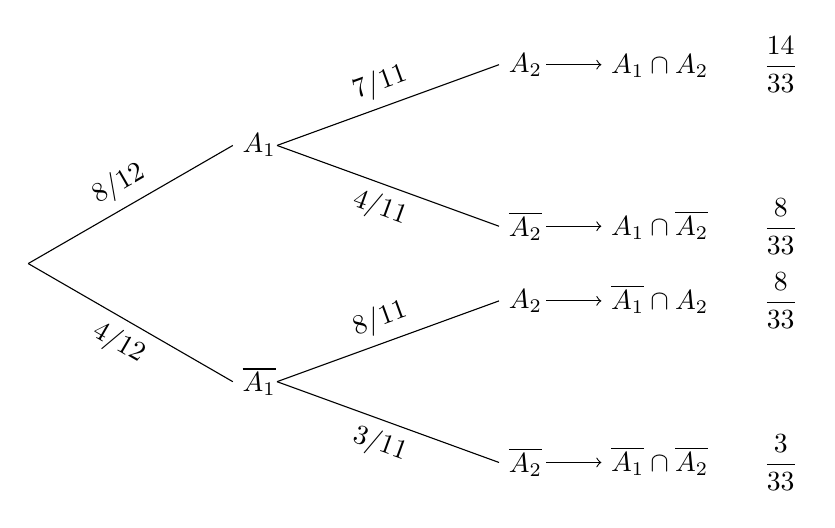
\begin{tikzpicture}

\draw (0,0) -- (30:3) node [right,] {$A_1$} node [above, midway, rotate=30, ] {$8/12$};
\draw (0,0) -- (-30:3) node [right, ] {$\overline{A_1}$} node [below, midway, rotate=-30, ] {$4/12$};
\draw (3.159807,1.5) -- ++(20:3) node [right, ] {$A_2$} node [above, midway, rotate=20, ] {$7/11$};
\draw (3.159807,1.5) -- ++(-20:3) node [right, ] {$\overline{A_2}$} node [below, midway, rotate=-20, ] {$4/11$};
\draw (3.159807,-1.5) -- ++(20:3) node [right, ] {$A_2$} node [above, midway, rotate=20, ] {$8/11$};
\draw (3.159807,-1.5) -- ++(-20:3) node [right, ] {$\overline{A_2}$} node [below, midway, rotate=-20, ] {$3/11$};
\draw [->] (6.57888,2.5260) -- ++(0:0.7) node [right, ] {$\displaystyle{A_1 \cap A_2 \qquad \frac{14}{33}}$};
\draw [->] (6.57888,0.4739) -- ++(0:0.7) node [right, ]   {$\displaystyle{A_1 \cap \overline{A_2} \qquad \frac{8}{33}}$};
\draw [->] (6.57888,-0.4739) -- ++(0:0.7) node [right, ]   {$\displaystyle{\overline{A_1} \cap A_2 \qquad \frac{8}{33}}$};
\draw [->] (6.57888,-2.5260) -- ++(0:0.7) node [right, ]   {$\displaystyle{\overline{A_1} \cap \overline{A_2} \qquad \frac{3}{33}}$};
\end{tikzpicture}
\caption{Diagrama de árvore indicando os quatro casos possíveis após o sorteio}
\label{arvore3}
\end{figure}

Logo, pela árvore, \(\displaystyle P(E)=\frac{8}{33}+\frac{8}{33}=\frac{16}{33}\).
\end{example}


\subsection{Eventos Independentes}

Na Atividade \emph{usio de óculos e sexo de estudantes}, concluímos que uso de óculos independe de gênero, pois  comparando as probabilidades incondicionais de ser do gênero feminino $(0,55)$ e de ser do gênero masculino $(0,45)$ com as probabilidades condicionais de ser do gênero feminino $(0,545)$ e do gênero masculino $(0,455)$ dado que usa óculos, percebe-se que elas são aproximadamente iguais. Na teoria, para que os eventos sejam independentes, essas probabilidades deveriam ser iguais. Na prática esse tipo de análise é usado em Estatística para avaliar a hipótese de independência entre dois eventos.
\begin{description}
\item[{Dois eventos \(A\) e \(B\) são ditos independentes\index{Dois eventos  e  são ditos independentes se a ocorrência de um deles não muda a incerteza sobre a ocorrência do outro.|textbf}}] se a ocorrência de um deles não muda a incerteza sobre a ocorrência do outro.
\end{description}

Em símbolos, \(A\) e \(B\)  são ditos eventos independentes se \(P(A|B)=P(A)\), ou equivalentemente, se \(P(B|A)=P(B)\).

Decorre, da definição de probabilidade condicional,
\(P(A|B)=\displaystyle\frac{P(A\cap B)}{P(B)}\), que se \(A\) e \(B\)
são eventos independentes, então \(P(A\cap B)=P(A) \cdot P(B)\).

É preciso ter cuidado ao usar este último resultado. Se não sabemos que os eventos \(A\) e \(B\) são independentes, então devemos usar a regra da multiplicação, a saber, \(P(A\cap B)=P(B)\cdot P(A|B)\) que vale para quaisquer dois eventos.

Observe que há uma simetria no conceito de independência de tal modo que se
\(P(A|B)=P(A)\), então \(P(B|A)=P(B)\).

De fato, se \(P(A|B)=P(A)\), segue que \(P(A\cap B)=P(A) \cdot P(B)\) e, assim,
\begin{equation*}
\begin{split}P(B|A)=\frac{P(A\cap B)}{P(A)}=\frac{P(A)\cdot P(B)}{P(A)}=P(B)\end{split}
\end{equation*}
\begin{example}{Eventos independentes versus eventos disjuntos}

Considere o experimento que consiste em lançar um dado honesto e, em seguida, lançar uma moeda honesta. Defina os eventos \(A:\) “ocorre uma face par” e \(B:\) “ocorre uma cara”.
\begin{enumerate}
\item {} 
\(A\) e \(B\) são eventos disjuntos?

\item {} 
\(A\) e \(B\) são eventos independentes?

\end{enumerate}

Observe que estamos lidando com um experimento sequencial de modo que os resultados possíveis envolvem a combinação de dois casos, a saber, número do dado e tipo de face da moeda. Como são seis números possíves para o dado e duas faces possíveis para a moeda, segue que o espaço amostral desse experimento consiste de 12 pares ordenados:

\(S=\{(1,ca),(1,co),(2,ca),(2,co),(3,ca),(3,co),(4,ca),(4,co),(5,ca),(5,co),(6,ca),(6,co)\}\)

Embora seja comum pensar que os eventos \(A\) e \(B\) são disjuntos, depois de descrever os elementos do espaço amostral é fácil perceber que $A$ e  $B$ não são disjuntos (\(A\cap B\neq \emptyset\)). De fato,
\begin{align*}
A&=\{(2,ca),(2,co),(4,ca),(4,co),(6,ca),(6,co)\}\text{, tal que } &P(A)&=\frac{6}{12}=0,5\\
B&=\{(1,ca),(2,ca),(3,ca),(4,ca),(5,ca),(6,ca)\} \text{, tal que } &P(B)&=\frac{6}{12}==0,5\\
A\cap B&=\{(2,ca),(4,ca),(6,ca)\} \text{, tal que }&P(A\cap B)&=\frac{3}{12}=\frac{1}{4}=0,25\\
\end{align*}

É natural pensarmos que os lançamentos do dado e da moeda sejam independentes, pois o resultado de um não interfere no resultado de outro. Podemos confirmar esse raciocínio, observando que \(P(A\cap B)=0,25\) é igual ao produto das probabilidades incondicionais de \(A\) e de \(B\)  ambas iguais a $0,5$.
\end{example}

Do exemplo anterior vale destacar que, dados dois eventos com probabilidade positiva, não será possível que eles sejam ao mesmo tempo disjuntos e independentes.

\begin{example} {Eventos disjuntos versus eventos independentes}

Sejam \(A\) e \(B\) dois eventos em um espaço amostral \(S\) tais que \(P(A)>0\) e \(P(B)>0\).
\begin{enumerate}
\item {} 
Se \(A\) e \(B\) são eventos disjuntos, então \(A\) e \(B\) não são eventos independentes.

Se \(A\) e \(B\) são disjuntos, então \(P(A\cap B)=0\neq P(A)\cdot P(B)>0\), pois \(P(A)>0\) e \(P(B)>0\). Assim, \(A\) e \(B\) não são independentes.

\item {} 
Se \(A\) e \(B\) são eventos independentes, então $A$ e $B$ não são eventos disjuntos.

Se \(A\) e \(B\) são independentes, então \(P(A\cap B)=P(A)\cdot P(B)>0\)o que implica que \(A\cap B\neq \emptyset\). Logo, \(a\) e \(B\) não são disjuntos.

\end{enumerate}

Observe que a única situação em que se pode ter \(A\)  e \(B\)  simultaneamente disjuntos e independentes ocorre se um dos eventos \(A\) ou \(B\) tiver probabilidade nula.
\end{example}

\begin{description}

\item[Três eventos \(A\), \(B\)  e  \(C\) são independentes] se, e somente se, eles são dois a dois independentes e \(P(A\cap B\cap C)=P(A)\cdot P(B)\cdot P(C)\).
\end{description}

\begin{example} {eventos dois a dois independentes não independentes}

Considere um dado em forma de tetraedro regular cujos números de suas faces são 1, 2, 3 e 4.

\begin{figure}[H]
\centering

\noindent\includegraphics[width=200bp]{{tetraedro_dado}.png}

\caption{Dado em forma de tetraedro com a face 2 oculta}
\end{figure}



Defina os eventos \(A=\{1,2\}\), \(B=\{1,3\}\) e \(C=\{1,4\}\).
\begin{enumerate}
\item {} 
Verifique que \(A\) e \(B\)  são eventos independentes.

\item {} 
Idem para \(A\) e \(C\).

\item {} 
Idem para \(B\) e \(C\).

\item {} 
Calcule \(P(A|B\cup C)\), compare o resultado obtido com \(P(A)\) e diga se \(A\) e \(B\cup C\) são eventos independentes.

\end{enumerate}

É fácil perceber que os eventos \(A\), \(B\) e \(C\) tomados dois a dois são independentes, pois a interseção entre dois dos três é sempre \(\{1\}\) cuja probabilidade é \(1/4\) e como cada um dos eventos \(A\), \(B\) e \(C\) têm probabilidade \(1/2\), segue que

\begin{align*}
P(A\cap B)&=P(A)\cdot P(B)=\frac{1}{2}\cdot\frac{1}{2}=\frac{1}{4}\\
P(A\cap C)&=P(A) \cdot P(C)=\frac{1}{2}\cdot\frac{1}{2}=\frac{1}{4} \\
P(B\cap C)&=P(B)\cdot P(C)=\frac{1}{2}\cdot\frac{1}{2}=\frac{1}{4}\\
\end{align*}

Mas, \(\displaystyle P(A|B\cup C)=\frac{P(A\cap (BUC))}{P(B\cup C)}=\frac{P((A\cap B)\cup (A\cap C))}{P(B\cup C)}=\frac{1/4}{3/4}=\frac{1}{3}\neq P(A)\) e, portanto, \(A\) e \(B\cup C\)  não são independentes apesar de \(A\) e \(B\) serem independentes e de \(A\) e \(C\) serem indepedentes.

Portanto, se temos três eventos dois a dois independentes, isso não implicará que os três eventos sejam independentes.
\end{example}


\practice{ Probabilidade Condicional}
\begin{task}{desempenho de exames diagnósticos}


Testes diagnósticos para detectar uma doença não são infalíveis. Para analisar o desempenho de um desses testes, realizam-se estudos em populações, contendo pessoas sãs e portadoras da doença.

\begin{figure}[H]
\centering

\noindent\includegraphics[width=200bp]{{amostras_sangue}.png}


\caption{Amostras de sangue para realização de exame}
\end{figure}


Quatro situações distintas podem ocorrer
\begin{enumerate}
\item {} 
a pessoa TEM a doença e o resultado do teste é POSITIVO.

\item {} 
a pessoa TEM a doença e o resultado do teste é NEGATIVO.

\item {} 
a pessoa NÃO TEM a doença e o resultado do teste é POSITIVO.

\item {} 
a pessoa NÃO TEM a doença e o resultado do teste é NEGATIVO.

\end{enumerate}

Observe que nas situações (b) e (c), o teste falha, pois deveria ser positivo quando a pessoa tem a doença e, negativo, quando a pessoa não tem a doença. Já nas situações (a) e (d) o teste acerta o diagnóstico.

Dois índices de desempenho para avaliação de um teste diagnóstico costumam ser usados: a sensibilidade e especificidade.

A \textbf{sensibilidade} é definida como a probabilidade de o resultado do teste ser POSITIVO, dado que a pessoa examinada tem a doença. Já a \textbf{especificidade} é a probabilidade do teste ser NEGATIVO, dado que a pessoa examinada não tem a doença.


O quadro a seguir refere-se a um teste diagnóstico para a doença \(X\), aplicado em uma amostra composta por duzentas pessoas, sendo 100 sadias e 100 portadoras da doença \(X\).

\begin{table}[H]
\centering
\begin{tabu} to \textwidth{|l|l|l|}
\hline
\thead
Resultado do teste & doente & sadia \\
\hline
Positivo & 95 & 15 \\
\hline
Negativo & 5 & 85 \\
\hline
\end{tabu}
\end{table}


Uma pessoa entre as duzentas dessa amostra será sorteada.
\begin{enumerate}
\item {} 
Qual a probabilidade de ela tenha a doença \(X\)?

\item {} 
Qual a probabilidade de que ela NÃO tenha a doença \(X\)?

\item {} 
Se o resultado do teste da pessoa sorteada foi positivo, calcule a probabilidade de que ela tenha a doença.

\item {} 
Se o resultado do teste da pessoa sorteada foi negativo, calcule a probabilidade de que ela tenha a doença.

\item {} 
Sabendo que a pessoa sorteada tem a doença, qual a probabilidade de seu teste ter resultado positivo?

\item {} 
Sabendo que a pessoa sorteada  NÃO tem a doença, qual a probabilidade de seu teste ter resultado negativo?

\item {} 
Determine uma estimativa da sensibilidade e da especificidade desse teste, usando a informação do quadro acima.

\end{enumerate}

\end{task}

\begin{task}{produção de peças}


\begin{figure}[H]
\centering

\noindent\includegraphics[width=400bp]{maquinas}

\caption{Produção de peças}
\end{figure}



Para fins de controle de qualidade das peças produzidas em uma fábrica, foram analisadas amostras de peças produzidas por máquinas diferentes. Os resultados obtidos estão resumidos no quadro a seguir.

\begin{table}[H]
\centering
\begin{tabu} to \textwidth{|c|c|c|}
\hline
\thead
Máquina
&
Defeituosas
&
Boas
\\
\hline
I
&
5
&
195
\\
\hline
II
&
15
&
585
\\
\hline
\end{tabu}
\end{table}


Pela informação das amostras coletadas, há razão para se acreditar que a produção de defeituosas ou boas é independente do tipo de máquina utilizada na produção?
\end{task}

\begin{task}{independência e complementariedade}


Sejam \(A\) e \(B\) dois eventos independentes.  Mostre que os pares de eventos a seguir também são independentes:
\begin{enumerate}
\item {} 
\(\overline{A}\) e \(\overline{B}\);

\item {} 
\(A\) e \(\overline{B}\); e

\item {} 
\(\overline{A}\) e \(B\).

\end{enumerate}
\end{task}

\begin{task}{escolha da chave correta}


\begin{figure}[H]
\centering
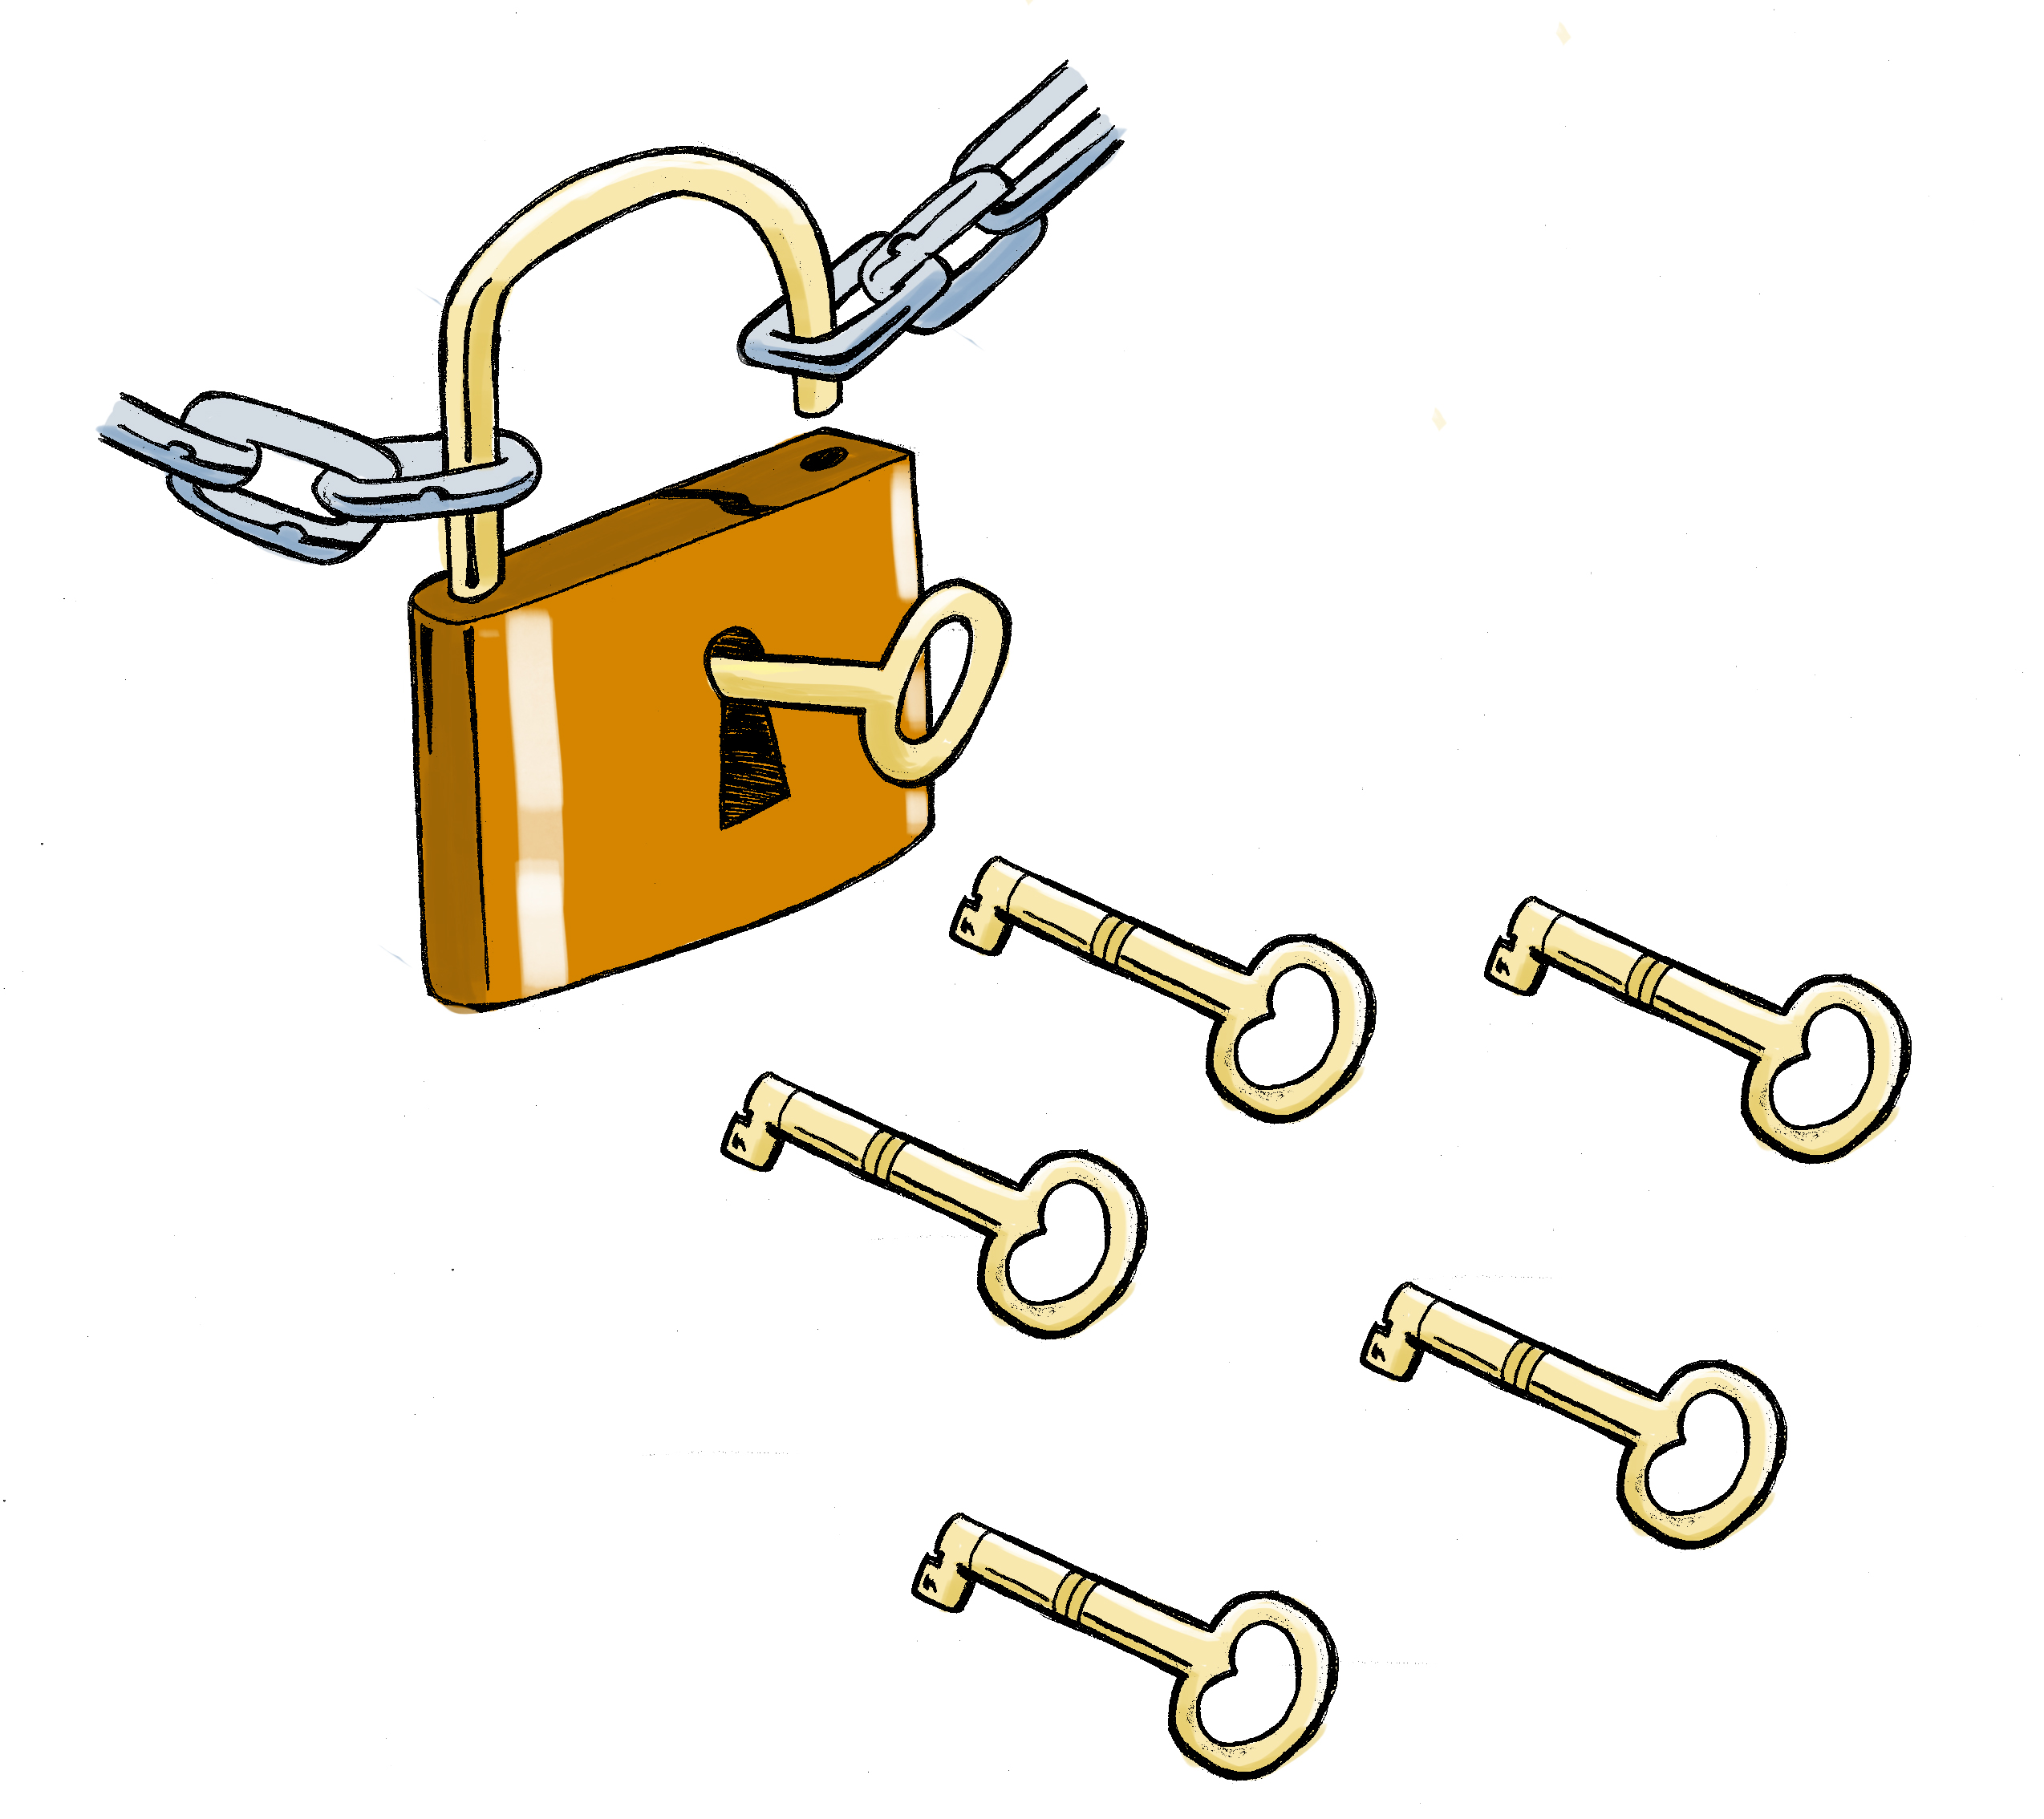
\includegraphics[width=200bp]{cadeado}

\caption{Chaves e cadeado}
\label{}
\end{figure}
Retirando-se chaves sequencialmente da caixa, qual a probabilidade de se abrir o cadeado apenas na terceira tentativa se:
\begin{enumerate}
\item a cada tentativa a chave extraída é recolocada na caixa?
\item a cada tentativa a chave extraída não é recolocada na caixa?
\item Em qual dos contextos (a) e (b) a probabilidade de se abrir a caixa é maior? Por quê?
\end{enumerate}

\end{task}

\begin{task}{probabilidade total}


Em um condomínio há três prédios: bloco I, bloco II e bloco III. No bloco I há 180 moradores, no bloco II há 200 moradores e no bloco III há 120 moradores. Entre os moradores do bloco I, há 27 menores de até 12 anos. Entre os moradores do bloco II há 36 menores de até 12 anos. Entre os moradores do bloco III há 24 menores de até 12 anos. Um residente do condomínio será sorteado da seguinte forma: primeiro será sorteado um bloco, tendo os blocos probabilidades iguais.  Depois, um residente do bloco sorteado será escolhido ao acaso, usando-se um cadastro dos moradores do bloco. Pede-se calcular a probabilidade
\begin{enumerate}
\item {} 
a probabilidade de que a pessoa sorteada seja um menor de até 12 anos;

\item {} 
a probabilidade de ter sido sorteado o bloco II, sabendo que a pessoa sorteada é um menor de até 12 anos.
  
\end{enumerate}

\begin{figure}[H]
\centering

\noindent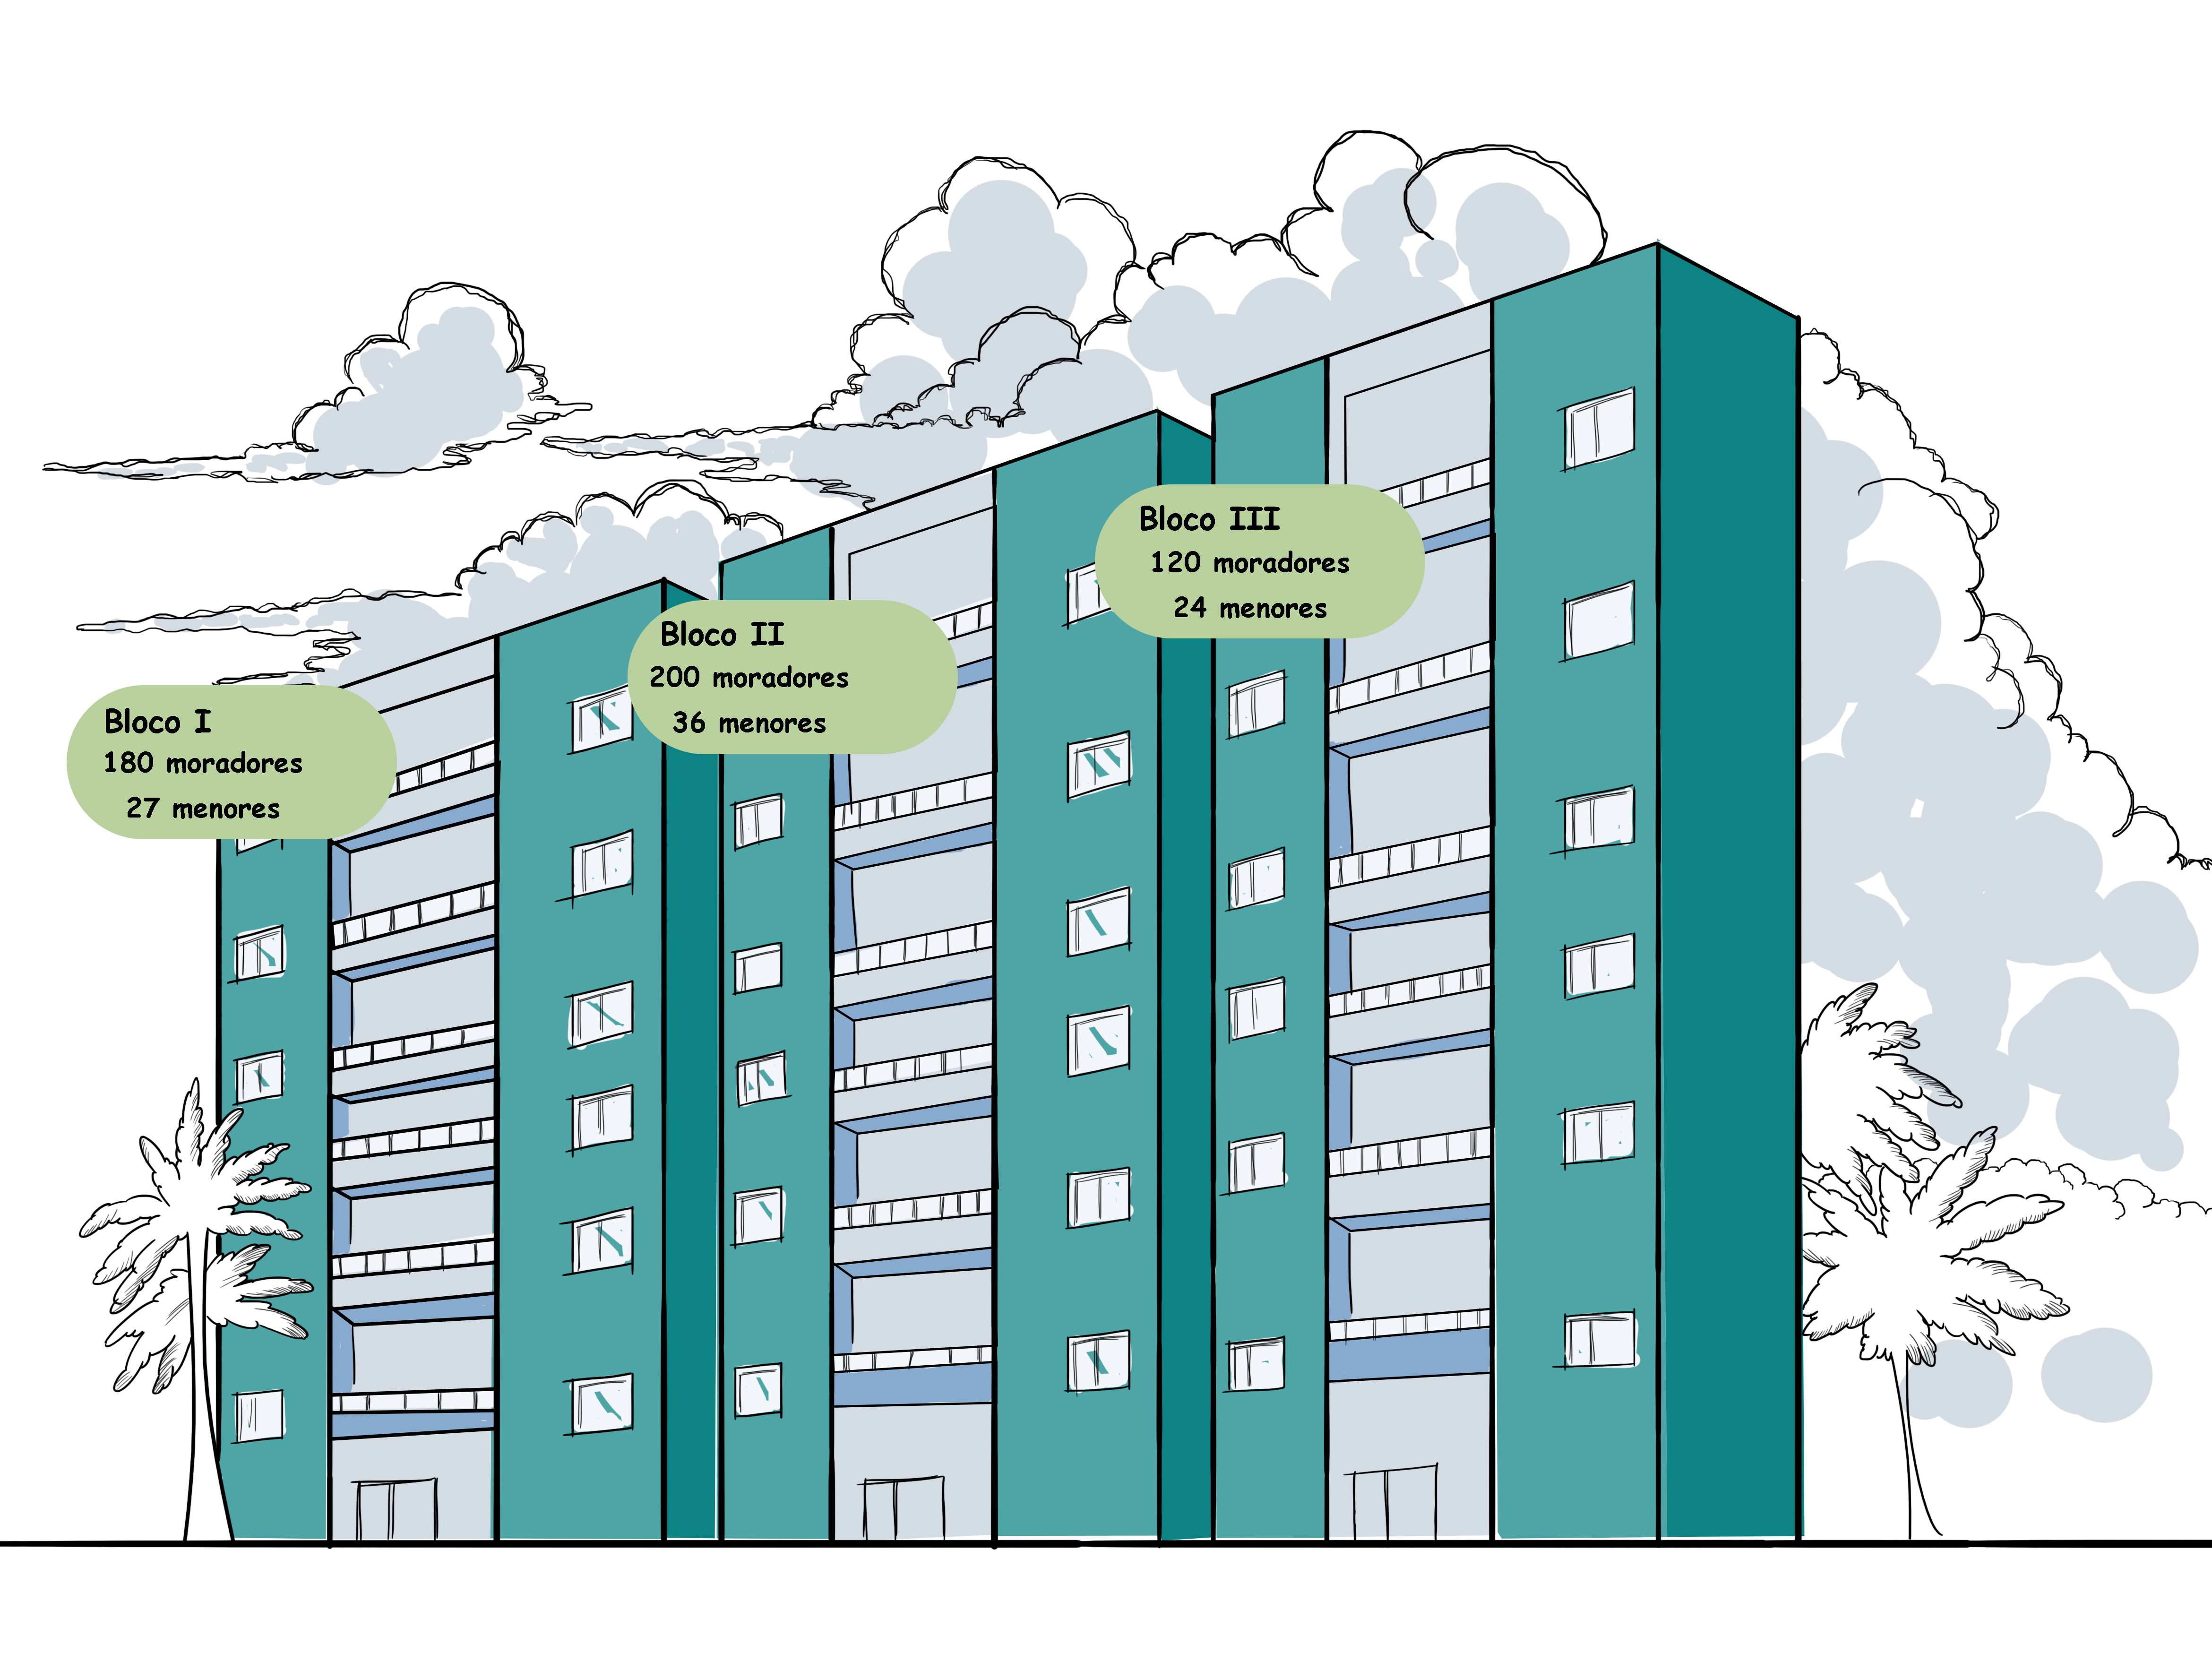
\includegraphics[width=400bp]{5.jpg}

\caption{Condomínio com três blocos}
\end{figure}

\end{task}
\know{ }

Em atividades anteriores foi sugerido lançar uma moeda repetidas vezes e registrar o resultado observado.  Veremos nesta seção como simular o lançamento de uma moeda um grande número de vezes com o auxílio da tecnologia.

Todos as linguagens de programação de computadores, planilhas e aplicativos costumam ter uma função interna usada para a geração de números aleatórios, na verdade, números pseudo-aleatórios, pois existe um mecanismo determinístico por trás da geração desses números.  Para mais detalhes sobre números (pseudo) aleatórios sugerimos assistir ao vídeo nesse  \href{https://www.youtube.com/watch?v=f4sE1r3UL4E}{link}.

Nessa seção serão apresentadas algumas ferramentas úteis para fazer simulações de experimentos simples como o lançamento de uma ou mais moedas e  o lançamento de um ou mais dados.

Uma simulação de um experimento é um processo que tem o mesmo comportamento do experimento, de tal modo que resultados similares à realidade sejam gerados pelo processo.

As atividades a seguir consistirão em simulações de fenômenos aleatórios simples. Para sua realização será necessário o uso de tecnologia. A seguir, duas possibilidades serão detalhadas: as planilhas do  \href{https://pt-br.libreoffice.org/}{LibreOffice} e do \href{https://wiki.geogebra.org/en/Reference:GeoGebra\_Installation}{GeoGebra}.

A função \emph{=ALEATÓRIOENTRE(1;N)} do LibreOffice, com \(N\) um número natural, produz um número do conjunto \(\{1,2,3,,\cdots, N\}\) de tal modo que a probabilidade de cada um dos números é dada por \(\frac{1}{N}\). Assim, ao usarmos \emph{=ALEATÓRIOENTRE(1;2)}, o resultado será equivalente a sortear um número do conjunto \(\{1,2\}\) cada um com probabilidade igual a \(\frac{1}{2}\). Veja na \hyperref[simulacao1]{figura \ref{simulacao1}} uma simulação de 20 números com essa propriedade, usando o LibreOffice.

\begin{figure}[H]
\centering

\noindent\includegraphics[width=400bp]{{libreoffice1}.png}

\caption{Vinte simulações do sorteio dos números 1 e 2 com probabilidades iguais, usando o LibreOffice}
\label{simulacao1}
\end{figure}
 

Para simular os 20 números, basta digitar na célula A1 \emph{=aleatórioentre(1;2)} e apertar a tecla \emph{Enter}. Depois, posicione o cursor no canto esquerdo inferior da célula e arraste para baixo até a linha 20. Os 20 números gerados neste exemplo estão na coluna A da planilha. É possível gerar rapidamente, muito mais do que apenas 20 números.

Essa função, \emph{aleatórioentre(1;2)} pode ser usada para simular o lançamento de uma moeda honesta, associando, por exemplo, o número 1 para a ocorrência de “cara” e, o número 2 para a ocorrência de  “coroa”, pois o modelo probabilístico da função \emph{=aleatórioentre(1;2)} é tal que os dois números são gerados com probabilidades iguais. Assim, espera-se, em média, que as quantidades de números 1 (1’s) e de números 2 (2’s) sejam aproximadamente iguais.

Como fazer para obter de forma rápida essas quantidades, sem ter que contar um a um?

No LibreOffice a função \emph{=cont.se(lista de células; número pesquisado)} faz essa contagem.

No exemplo anterior, a função \emph{=cont.se(A1:A20;1)} irá retornar o número de 1’s encontrados nas células da coluna A das linhas 1 a 20. Já a  a função \emph{=cont.se(A1:A20;2)} irá retornar o número de 2’s encontrados nas células da coluna A das linhas 1 a 20. Veja uma ilustração do uso da função na \hyperref[simulacao2]{figura \ref{simulacao2}}. Nessa figura, vemos que na simulação foram gerados doze (12) números 1 (caras) e oito (8) números 2 (coroas).

\begin{figure}[H]
\centering

\noindent\includegraphics[width=400bp]{{Libreoffice2}.png}

\caption{Exemplo do uso da função cont.se do LibreOffice}
\label{simulacao2}
\end{figure}

 

No Geogebra as funções para realizar as mesmas tarefas são similares às utilizadas no LibreOffice. Veja na \hyperref[simulacao3]{figura \ref{simulacao3}} a simulação do lançamento de uma moeda honesta 20 vezes, usando a função \emph{=NúmeroAleatório(1,2)} do GeoGebra.

\begin{figure}[H]
\centering

\noindent\includegraphics[width=400bp]{{GeoGebra1_1}.png}
\caption{GeoGebra: simulação de 20 lançamentos de uma moeda honesto, associando 1 para cara e 2 para coroa}
\label{simulacao3}
\end{figure}


Para a realização da contagem de caras e coroas, a função correspondente no GeoGebra é a função \emph{ContarSe(números, células)}.

A quantidade de 1’s na coluna A das linhas 1 a 20 é dada por \emph{=ContarSe(0\textless{}x\textless{}2,A1:A20)} que produzirá a quantidade de números inteiros no intervalo aberto {]}0,2{[} que ocorrem nas celas da coluna A das linhas 1 a 20 (A1:A20). Observe que o único número inteiro no intervalo aberto {]}0,2{[} é o número 1. Para contar a quantidade de 2’s na coluna A, devemos digitar \emph{=ContarSe(1\textless{}x\textless{}3,A1:A20)}, lembrando que o único número inteiro no intervalo aberto {]}1,3{[} é o número 2.

\begin{figure}[H]
\centering

\noindent\includegraphics[width=400bp]{{GeoGebra2_1}.png}

\caption{Geogebra: exemplo de uso da função \emph{ContarSe}}
\end{figure}


Observe que na simulação realizada com o GeoGebra também foram obtidos doze números 1 (caras) e oito (8) números 2 (coroas). De fato, trata-se de mera coincidência, pois espera-se que, em média sejam produzidos a cada simulação, 10 caras.

\begin{example}{experimento cujo espaço amostral é equiprovável.}

Suponha que o espaço amostral \(S\) é dado por \(\{ 1,2,3,4,5,6,7,8,9,10,11,12\}\) e que os eventos elementares são equiprováveis.

A função do LibreOffice \emph{=AleatórioEntre(1;12)} retornará com probabilidade \(\frac{1}{12}\) um dos elementos de \(S\).

A função do GeoGebra \emph{=NúmeroAleatório(1,12)} retornará com probabilidade \(\frac{1}{12}\) um dos elementos de \(S\).

\begin{figure}[H]
\centering

\noindent\includegraphics[width=400bp]{{geo1_1}.png}

\caption{Funções no Geogebra e LibreOffice}
\end{figure}

Observação:  Você poderá simular o lançamento de um dado ou de mais de um dado honesto e muitos outros experimentos simples, usando essas funções do Geogebra e do LibreOffice.
\end{example}
\begin{task}{simulação do lançamento de uma moeda honesta}


Deseja-se simular o lançamento de uma moeda honesta uma grande quantidade de vezes e comparar a frequência relativa de caras com a probabilidade teórica 0,5 de obter uma cara quando a moeda é honesta.

\begin{figure}[H]
\centering

\noindent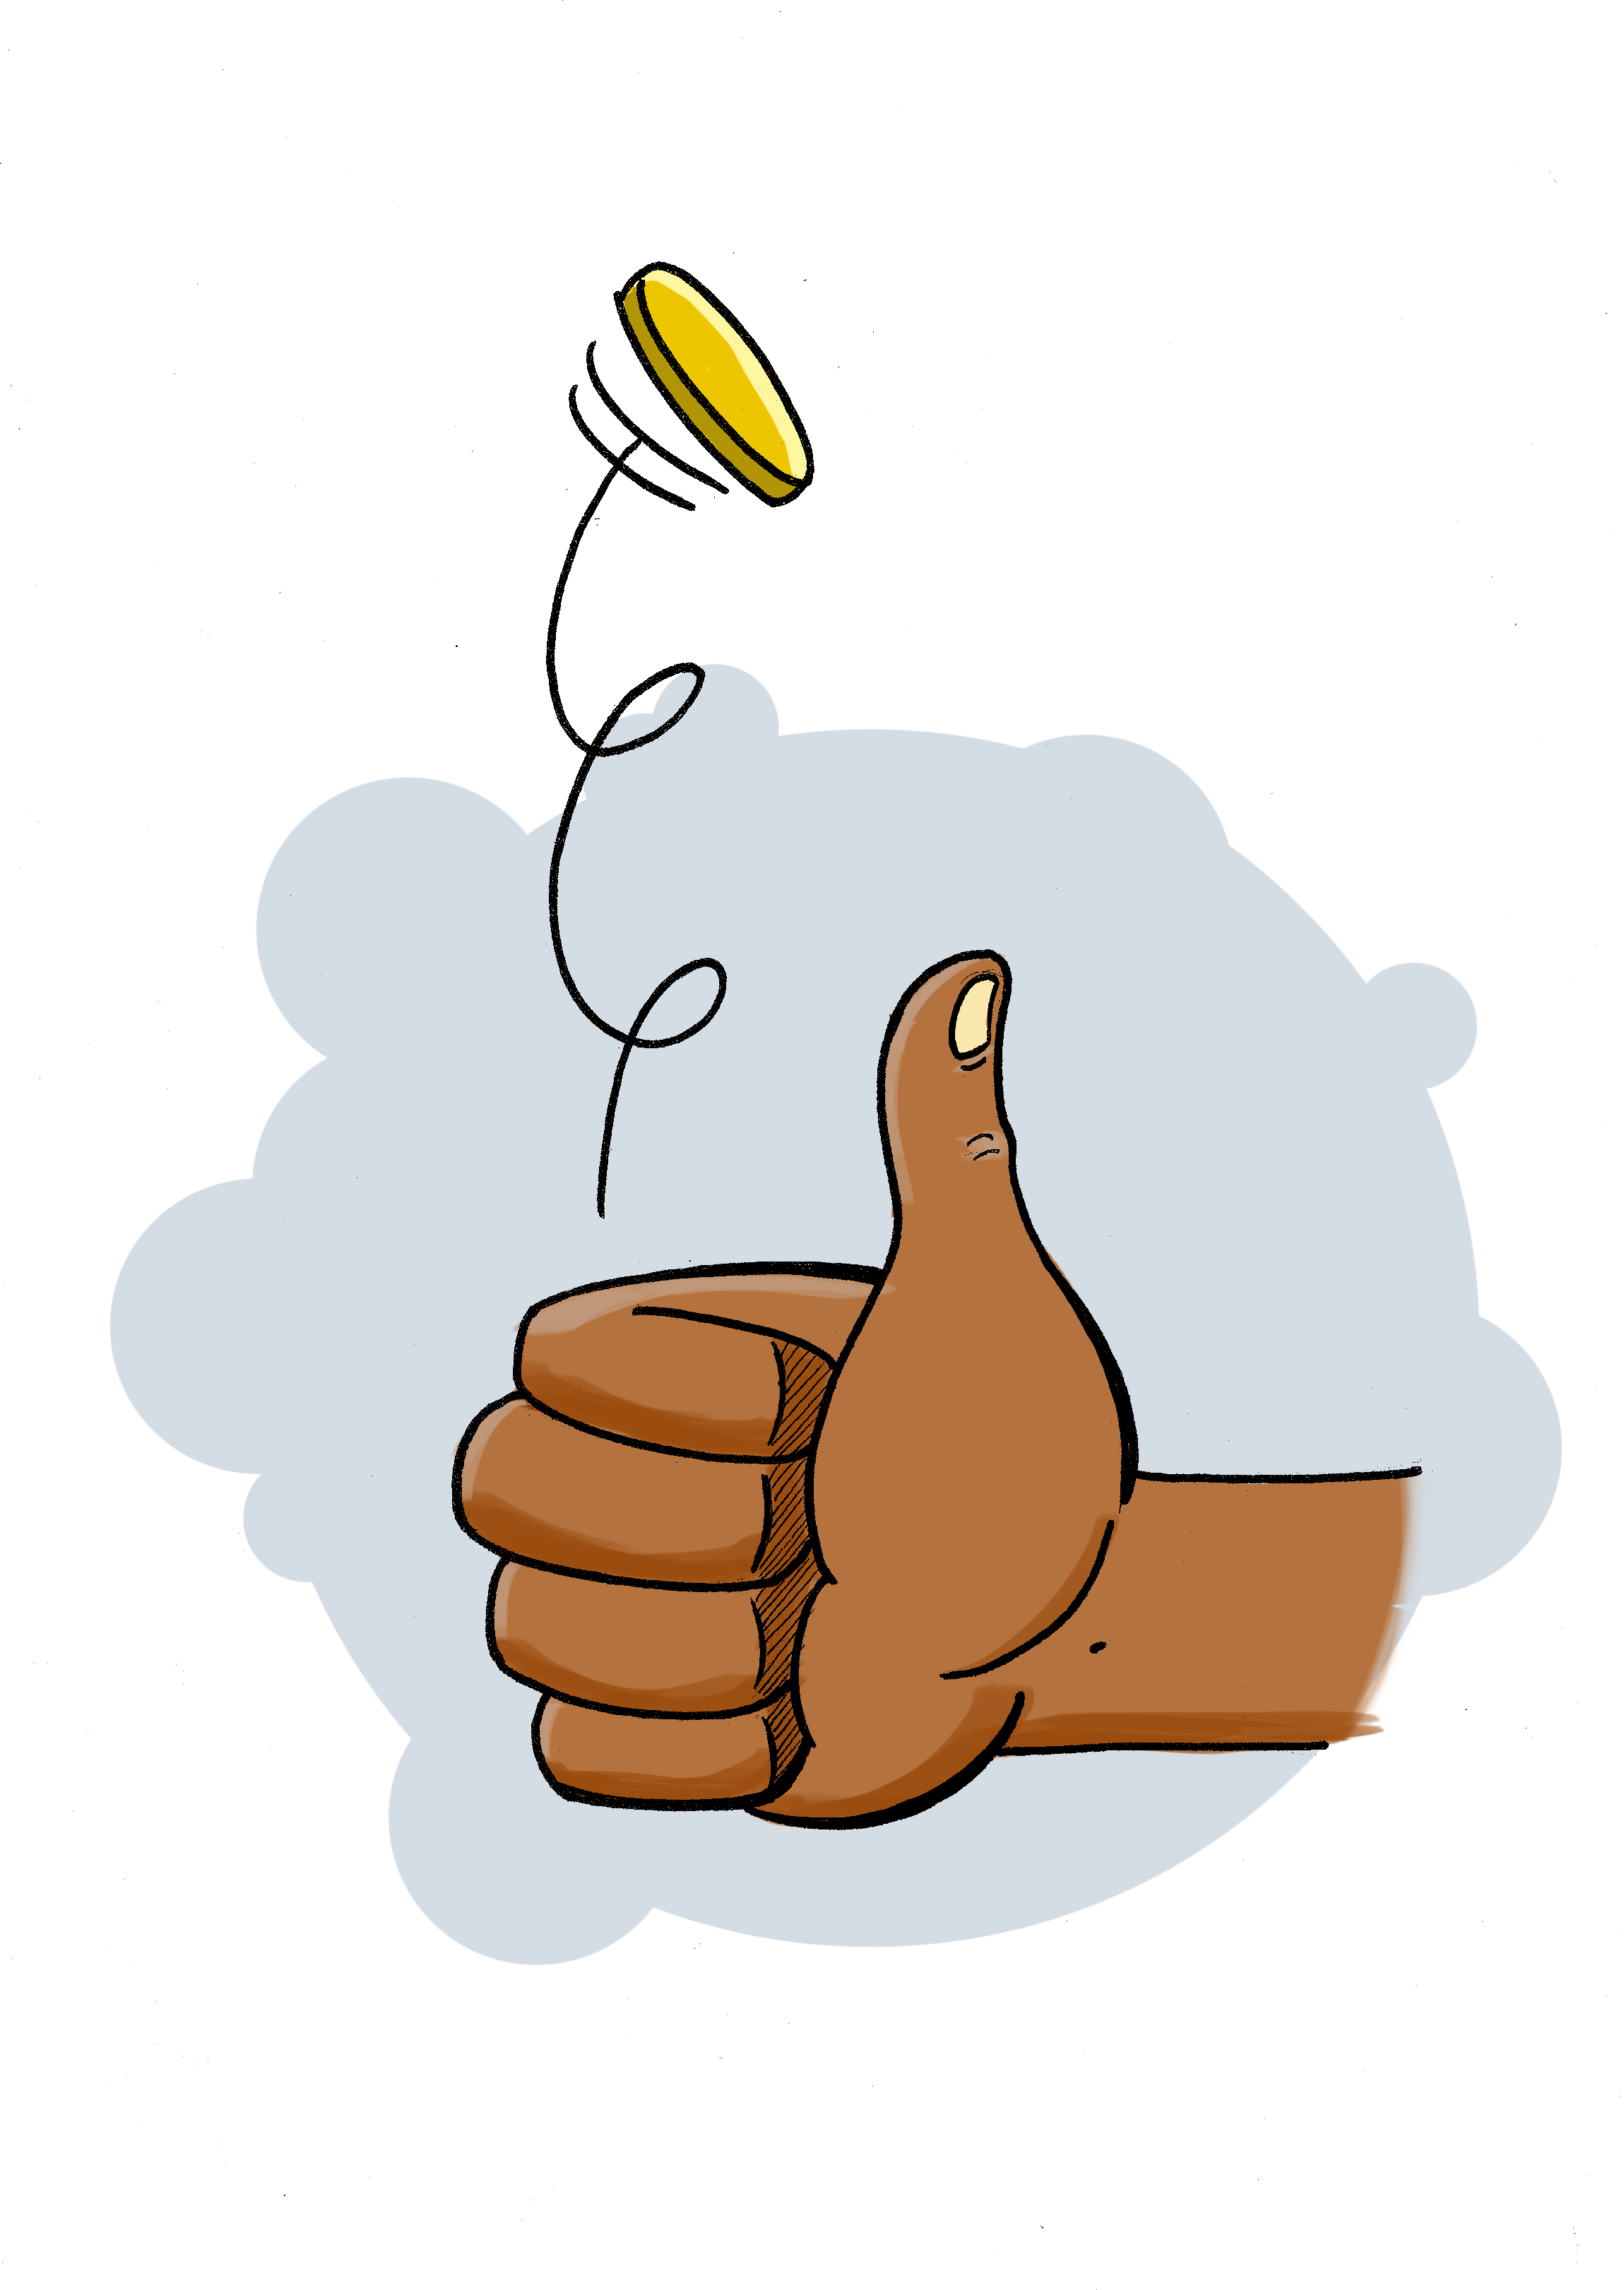
\includegraphics[width=150bp]{moeda.jpg}
\end{figure}
\begin{enumerate}
\item {} 
Usando o GeoGebra ou algum outro recurso tecnológico, simule 20 lançamentos da moeda e observe a quantidade de caras, calculando a frequência relativa.

\item {} 
Repita a simulação para 50, 100, 250 e 1000 lançamentos da moeda.

\item {} 
Complete o quadro a seguir e comente sobre os resultados obtidos.

\end{enumerate}

\begin{table}[H]
\centering
\begin{tabu} to \textwidth{|c|c|}
\hline
\thead
Número de Observações & Frequência relativa de caras \\
\hline
20 &\\
\hline
50 &\\
\hline
100 &\\
\hline
250 &\\
\hline
1000 &\\
\hline
\end{tabu}
\end{table}

\end{task}

\begin{task}{simulação do lançamento de um dado honesto}


Deseja-se simular o lançamento de um dado honesto uma grande quantidade de vezes e comparar a frequência relativa de faces “6” com a probabilidade teórica \(\frac{1}{6}\approx 0,167\) de obter uma face “6” quando o dado é honesto.

\begin{figure}[H]
\centering

\noindent\includegraphics[width=200bp]{{lancamento_dado}.png}
\end{figure}
\begin{enumerate}
\item {} 
Usando o GeoGebra ou algum outro recurso tecnológico, simule 30 lançamentos do dado e observe a quantidade de faces “6” obtidas, calculando a frequência relativa.

\item {} 
Repita a simulação para 60, 120, 300 e 1500 lançamentos do dado.

\item {} 
Complete o quadro a seguir e comente sobre os resultados que você obteve.

\end{enumerate}
\begin{table}[H]
\centering
\begin{tabu} to \textwidth{|c|c|}
\hline
\thead
\centering
Número de Observações & Frequência relativa de 6 \\
\hline
30 &\\
\hline
60 &\\
\hline
120 &\\
\hline
300 &\\
\hline
1500 &\\
\hline
\end{tabu}
\end{table}
\end{task}

\begin{task}{simulação do lançamento de um dado desequilibrado}


Um dado é desequilibrado quando suas faces ocorrem com probabilidades desiguais. Suponha que um dado seja desequilibrado de tal modo que a probabilidade de ocorrer cada uma de suas faces, entre os números 1, 2, 3, 4, 5 e 6, sejam proporcionais aos respectivos números das faces.
\begin{enumerate}
\item {} 
Determine as probabilidades de cada face no caso desse dado.

\item {} 
Usando as funções de geração de números aleatórios, simule o lançamento desse dado 42 vezes e compare a frequência relativa de faces 6 obtidas com a probabilidade teórica da face 6 obtida no item anterior.

\item {} 
Repita o item anterior para 84, 210, 630, 840 e 1680 lançamentos do dado desequilibrado e registre o número de vezes que você obteve a face 6.

\item {} 
Complete a tabela a seguir e comente sobre os resultados que você obteve.

\end{enumerate}

\begin{table}[H]
\centering
\begin{tabu} to \textwidth{|c|c|}
\hline
\thead
Número de Observações & Frequência relativa de 6 \\
\hline
42 &\\
\hline
210 &\\
\hline
630 &\\
\hline
840 &\\
\hline
1680 &\\
\hline
\end{tabu}
\end{table}

\end{task}

\begin{task}{simulação do lançamento de um dado diferente}


Um dado é equilibrado, mas suas faces foram pintadas de tal modo que há uma face 1, duas faces 2 e três faces 3.
\begin{enumerate}
\item {} 
Determine as probabilidades de se obter face 1, face 2 e face 3 com esse dado.

\item {} 
Usando as funções de geração de números aleatórios, simule o lançamento desse dado 30 vezes e compare a frequência relativa de faces 2 obtidas com a probabilidade teórica da face 2 obtida no item anterior.

\item {} 
Repita o item anterior para 300, 600, 900 e 1800 lançamentos do dado equilibrado e registre o número de vezes que você obteve a face 2.

\item {} 
Complete a tabela a seguir e comente sobre os resultados que você obteve.

\end{enumerate}

\begin{table}[H]
\centering
\begin{tabu} to \textwidth{|c|c|}
\hline
\thead
Número de Observações & Frequência relativa de 2 \\
\hline
30 &\\
\hline
300 &\\
\hline
600 &\\
\hline
900 &\\
\hline
1800 &\\
\hline
\end{tabu}
\end{table}
\end{task}

\begin{observation}{Teorema: Lei dos Grandes Números}

À medida que um experimento é repetido várias vezes, a probabilidade dada pela frequência relativa de um evento tende a se aproximar da probabilidade teórica.
\end{observation}

A lei dos grandes números nos diz que as estimativas da probabilidade de um evento dadas pelas frequências relativas tendem a ficar melhores com mais observações. Esse resultado, como já comentado anteriormente, é a base teórica para a interpretação frequentista de probabilidade. Veja na \hyperref[1000_lancamentos2]{figura \ref{1000_lancamentos2}}, uma ilustração da Lei dos Grandes Números.

\begin{example}{Cálculo de probabilidade, usando simulação}

Deseja-se calcular a probabilidade de se obter pelo menos uma face 6, quando um dado honesto é lançado quatro vezes.

Definindo \(A\) como sendo o evento ocorreu pelo menos um seis nos quatro lançamentos, então \(\overline{A}\) é o evento nenhum 6 ocorreu nos quatro lançamentos.

Nesse caso, podemos usar a propriedade do evento complementar para calcular \(P(A)=1-P(\overline{A})\).
O evento \(\overline{A}\)  ocorre se, e somente se, em cada um dos quatro lançamentos não ocorre face 6. Como os lançamentos são independentes, a probabilidade de não ocorrer face 6 nos quatro lançamentos será dada por
\begin{equation*}
\begin{split}\frac{5}{6}\cdot \frac{5}{6}\cdot \frac{5}{6}\cdot \frac{5}{6}=\left (\frac{5}{6}\right )^4\approx 0,48\end{split}
\end{equation*}
Assim \(P(A) \approx 1- 0,48=0,52\).

Vamos estimar essa probabilidade, usando a Lei dos Grandes Números com o auxílio do GeoGebra.

Para simular o experimento podemos usar a função \emph{=Número Aleatório(1,6)} nas céluas A1 até A4.

\begin{figure}[H]
\centering

\noindent\includegraphics[width=370bp]{{GeoGebra_e1}.png}

\caption{Simulação de quatro lançamento de um dado com o GeoGebra}
\end{figure}

\hyperref[geogebra2]{figura \ref{geogebra2}}: Simulação de quatro lançamento de um dado com o GeoGebra

Na cela B4 usaremos a função \emph{=ContarSe(5\textless{}x\textless{}7,A1:A4)} para obter o número de faces 6 obtidas.

\begin{figure}[H]
\centering

\noindent\includegraphics[width=370bp]{{GeoGebra_e2}.png}
\caption{Contagem do número de faces 6 obtidas, usando o GeoGebra}
\label{geogebra2}
\end{figure}


Depois, marque as células A1:B4 e arraste-as até a linha 400, de modo a repetir 100 vezes esse experimento.

\begin{figure}[H]
\centering

\noindent\includegraphics[width=370bp]{{GeoGebra_e3_1}.png}

\caption{Simulação de 100 experimentos (lançar um dado 4 vezes), usando o GeoGebra}
\end{figure}


Vamos então usar a função \emph{ContarSe(-1\textless{}x\textless{}1,B1:B400)} para obter a quantidade de zeros, ou seja, o número de repetições do experimento em que a face 6 não ocorreu.

\begin{figure}[H]
\centering

\noindent\includegraphics[width=400bp]{{GeoGebra_e4_1}.png}

\caption{Contagem do número de ocorrências do evento “nenhuma face 6”}
\end{figure}


Observe que foram 43 ocorrências sem nenhuma face 6 de modo que nessa simulação a probabilidade estimada de obter pelo menos um 6 é dada por \(1-0,43=0,57\). Observe que essa estimativa ficou ligeiramente afastada da probabiliade teórica (\(\approx 0,52\)).

Duplicando o número de repetições do experimento, espera-se obter uma estimativa mais próxima da probabilidade teórica. Veja na \hyperref[geogebra5]{figura \ref{geogebra5}} um resultado, usando o GeoGebra. Agora, com 200 repetições, a estimativa  foi $0,54$ e, portanto, mais perto da probabilidade teórica.

\begin{figure}[H]
\centering

\noindent\includegraphics[width=400bp]{{GeoGebra_e5}.png}

\caption{Simulação de 200 experimentos (lançar um dado 4 vezes), usando o GeoGebra}
\label{geogebra5}
\end{figure}

\end{example}


\exercise

\begin{enumerate}

\item (Pisa) Imagine que tenha sido apresentado um documentário sobre terremotos, no qual é dito com que frequência ocorrem  e como podem ser previstos. Nesse documentário, um geólogo afirmou: “nos próximos  20 anos, a chance de um terremoto acontecer na cidade de Zed é de duas em três.”

Qual das sentenças a seguir reflete o significado da afirmação feita pelo geólogo?
\begin{enumerate}
\item {} 
Como \(\frac{2}{3}\cdot 20\approx 13,3\); entre 13 e 14 anos a partir de agora, ocorrerá um terremoto na cidade de Zed.

\item {} 
Como \(\frac{2}{3}\) é maior do que \(\frac{1}{2}\), temos certeza de que ocorrerá um terremoto na cidade de Zed em algum momento nos próximos 20 anos.

\item {} 
A probabilidade de ocorrer algum terremoto na cidade de Zed em algum momento nos próximos 20 anos é maior do que a probabilidade de ele não ocorrer.

\item {} 
Não se pode dizer sobre o que irá acontecer, pois ninguém sabe quando um terremoto ocorrerá.

\end{enumerate}

\item (Pisa) Para dado dia, a previsão do tempo afirma que, das 12h às 18h, a chance de ocorrência de chuva é de 30\%.

Assinale a alternativa que corresponde à melhor interpretação dessa previsão do tempo.
\begin{enumerate}
\item {} 
Em 30\% da área à qual a previsão se refere haverá chuva.

\item {} 
em 30\% de 6 horas, ou seja, durante o total de 108 minutos, haverá chuva.

\item {} 
Em relação às pessoas da área à qual a previsão se refere, pode-se afirmar que 30 a cada 100 pessoas pegarão chuva.

\item {} 
Se a mesma previsão fosse dada para 100 dias, em cerca de 30 desses 100 dias haveria chuva.

\item {} 
A quantidade de chuva será 30\% da intensidade de uma forte precipitação (medida como “chuva por unidade de tempo”).

\end{enumerate}

\item Sabe-se que a probabilidade de que um casal com três filhos tenha duas meninas é \(\frac{3}{8}\). Com base nessa afirmação, responda:
\begin{enumerate}
\item {} 
Observando-se ao acaso 160 casais com três filhos, quantos casais você espera que tenham duas meninas?

\item {} 
E em 400 casais com três filhos?

\item {} 
É correto afirmar que se observarmos 80 casais com três filhos, exatamente 30 casais terão duas meninas? Por quê?

\end{enumerate}

\item Nas situações a seguir indique a interpretação de probabilidade, entre as interpretações clássica, frequentista e subjetiva, que melhor se encaixa para a designação de probabilidades.
\begin{enumerate}
\item {} 
Um dado honesto é lançado três vezes, deseja-se calcular a probabilidade de se obter pelo menos duas faces pares.

\item {} 
Um gerente de banco deseja avaliar a probabilidade de um cliente esperar mais de 30 minutos para ser atendido em um dia comum.

\item {} 
Deseja-se avaliar a probabilidade de você se tornar um \emph{Youtuber} de sucesso no próximo ano.

\end{enumerate}

\item Em uma escola de Ensino Médio há dois turnos: manhã e tarde. Nesta escola há alunos que praticam atividade física fora do horário escolar e alunos que não praticam. Um aluno dessa escola será sorteado. Defina os seguintes eventos \(A:\) “o aluno sorteado é do turno da manhã” e \(B:\) “o aluno sorteado pratica atividade física fora do horário escolar”. Descreva em palavras os eventos
\begin{enumerate}
\item {} 
\(A\cup B\)

\item {} 
\(A\cap B\)

\item {} 
\(\overline{A}\cap \overline{B}\)

\item {} 
\(\overline{A\cap B}\)

\end{enumerate}

\item É sorteado um aluno de uma turma de um curso de Inglês na qual há somente alunos de 15 anos, 16 anos e 17 anos completos. Sabe-se que a  probabilidade de o aluno selecionado ter 15 anos é igual a 0,3 e ter 17 anos é igual a 0,2.
Determine a probabilidade de o aluno sorteado
\begin{enumerate}
\item {} 
ter idade maior do que 16 anos.

\item {} 
ter 16 anos.

\item {} 
ter pelo menos 15 anos.

\item {} 
ter 15 ou 16 anos.

\end{enumerate}

\item Um posto de coleta de sangue fez um lavantamento das fichas de 500 doadores, obtendo as seguintes frequências relativas por tipo sanguíneor e fator Rh.

\begin{table}[H]
\centering
\begin{tabu} to \textwidth{|c|c|c|c|}
\hline
\thead
tipo & Rh+ & Rh- & total \\
\hline
O & 0,32 & 0,08 & 0,40 \\
\hline
A & 0,20 & 0,10 & 0,30 \\
\hline
AB & 0,16 & 0,04 & 0,20 \\
\hline
B & 0,07 & 0,03 & 0,10 \\
\hline
total & 0,75 & 0,25 & 1,00 \\
\hline
\end{tabu}
\end{table}


Supondo que o comportamento desses doadores reflita o comportamento da população da região do posto de coleta que contém 1 milhão de pessoas, pede-se calcular, de forma aproximada, o número de pessoas nessa população que
\begin{enumerate}
\item {} 
tenha fator Rh-;

\item {} 
tenha sangue tipo A;

\item {} 
tenha sangue tipo AB com fator Rh+;

\item {} 
não tenha sangue tipo O.

\item {} 
não tenha sangue tipo O, sabendo que tem fator Rh+.

\item {} 
não tenha sangue tipo O, sabendo que tem fator Rh-.

\end{enumerate}

\item (UERJ-EQ1-2011) Uma fábrica produz sucos com os seguintes sabores: uva, pêssego e laranja. Considere uma caixa com 12 garrafas desses sucos, sendo quatro de cada sabor. Retirando-se ao acaso duas garrafas dessa caixa, a probabilidade de que ambas as garrafas contenham suco com o mesmo saber equivale a:
\begin{enumerate}
\item {} 
9,1\%

\item {} 
18,2\%

\item {} 
27,3\%

\item {} 
36,4\%

\end{enumerate}

\item (UERJ-EQ1-2012-adaptada) Três modelos de aparelhos de ar condicionado I, II e III, de diferentes potências são produzidos por determinado fabricante. Uma consulta sobre intenção de troca de modelo foi realizada com 1000 usuários desses produtos. No quadro a seguir estão indicados os tipos de modelos que os usuários possuem e se eles pretendem mudar para outro modelo ou não.

Dos 400 que possuem o modelo I, 50 não pretendem mudar de modelo, 150 pretendem mudar para o II e 250 para o III. Dos 400 que possuem o modelo II, 100 não pretendem mudar e 300 pretendem mudar para o III. E, dos 200 que possuem o modelo III, nenhum deles tem intenção de mudar.

Escolhendo-se aleatoriamente um dos usuários consultados, a probabilidade de que ele não pretenda trocar seu modelo de ar condicionado é:
\begin{enumerate}
\item {} 
20\%

\item {} 
35\%

\item {} 
40\%

\item {} 
65\%

\end{enumerate}

\item (UERJ-EQ2-2013) Em uma escola, 20\% dos alunos de uma turma marcaram a opção correta de uma questão de múltipla escolha que possui quatro alternativas de resposta. Ode demais alunos marcaram uma das quatro opções ao acaso. Verificando-se as respostas de dois alunos quaisquer dessa turma, a probabilidade de que exatamente um tenha marcado a opção correta é:
\begin{enumerate}
\item {} 
0,48

\item {} 
0,40

\item {} 
0,36

\item {} 
0,25

\end{enumerate}

\item (ENEM) Um aluno de determinada escola será escolhido por sorteio para representa-la em certa atividade. A escola tem dois turnos. No diurno há 300 alunos, distribuídos em 10 turmas de 30 alunos cada. No noturno há 240 alunos, distribuídos em 6 turmas de 40 alunos cada. Em vez do sorteio direto, envolvendo os 540 alunos, foram propostos dois outros métodos de sorteio.
MÉTODO I: Escolher ao acaso um dos turnos e, a seguir, sortear um dos alunos do turno escolhido.
MÉTODO II: Escolher ao acaso uma das 16 turmas e, a seguir, sortear um dos alunos dessa turma.
Sobre os métodos I e II é correto afirmar:
\begin{enumerate}
\item {} 
Em ambos os métodos, todos os alunos têm a mesma chance de serem sorteados.

\item {} 
No método I, todos os alunos têm a mesma chance de serem sorteados, mas no método II a chance de um aluno do diurno ser sorteado é maior do que a de um aluno do noturno.

\item {} 
No método II, todos os alunos têm a mesma chance de serem sorteados, mas no método I a chance de um aluno do diurno ser sorteado é maior do que a de um aluno do noturno.

\item {} 
No método I, a chance de um aluno do noturno ser sorteado é maior do que a chance de um aluno do diurno, enquanto no método II ocorre o contrário.

\item {} 
Em ambos os métodos, a chance de um aluno do diurno ser sorteado é maior do que a de um aluno do noturno.

\end{enumerate}

\item (ENEM) Um município de 628 km2 é atendido por duas emissoras de rádio cujas antenas A e B alcançam um raio de 10 km do município, conforme mostra a \hyperref[municipio]{figura \ref{municipio}}:
\begin{figure}[H]
\centering

\begin{tikzpicture}

\draw [color=secundario!70, fill=primario!70] (2,3) -- (3,3) -- (3.55,2.16);
\draw [dashed, ] (0,0) -- (0,3);
\draw [] (0,3) -- (3,3) -- (5,0) -- (0,0);
\draw [, fill=primario!70] (2,3) arc (-180:-56.1:1);
\draw [, fill=primario!70] (5,0) -- (4,0) arc (180:123.9:1) -- cycle;
\node [above right, ] at (3,3) {$A$};
\node [above, scale=0.8] at (2.5,3) {10 km};
\node [rotate=-56.1, above, scale=0.8] at (4.718, 0.395) {10 km};
\node [below right, ] at (5,0) {$B$};
\node [below, scale=0.8] at (4.5,0) {10 km};
\draw [very thin] (0,0) rectangle (0.2,0.2);
\draw [very thin] (0,3) rectangle (0.2,2.8);
\node [ponto] at (0.1,0.1) {};
\node [ponto] at (0.1,2.9) {};
\draw plot [smooth, tension=1] coordinates {(1,3) (0.75,1.5) (1.5,0)};
\node [right] at (1,1.5) {Município};
\end{tikzpicture}
\caption{Planta do município}
\label{municipio}
\end{figure}

Para orçar um contrato publicitário, uma agência precisa avaliar a probabilidade que um morador tem de, circulando livremente pelo município, encontrar-se na área de alcance de pelo menos uma das emissoras. Essa probabilidade é de aproximadamente:
\begin{enumerate}
\item {} 
20\%

\item {} 
25\%

\item {} 
30\%

\item {} 
35\%

\item {} 
40\%

\end{enumerate}

\item (ENEM - 2017) Um morador de uma região metropolitana tem 50\% de probabilidade de atrasar-se para o trabalho quando chove na região; caso não chova, sua probabilidade de atraso é de 25\%. Para um determinado dia, o serviço de meteorologia estima em 30\% a probabilidade da ocorrência de chuva nessa região.

Qual é probabilidade de esse morador se atrasar para o serviço no dia para o qual foi dada a estimativa de chuva?
\begin{enumerate}
\item {} 
0,075

\item {} 
0,150

\item {} 
0,325

\item {} 
0,600

\item {} 
0,800

\end{enumerate}

\item (ENEM - 2017) Numa avenida existem 10 semáforos. Por causa de uma pane no sistema, os semáforos ficaram sem controle durante uma hora, e fixaram suas luzes unicamente em verde ou vermelho. Os semáforos funcionam de forma independente; a probabilidade de acusar cor verde é de \(\frac{2}{3}\) e a de acusar cor vermelha é de \(\frac{1}{3}\). Uma pessoa percorreu a pé toda essa avenida durante o período da pane, observando a cor da luz de cada um desses semáforos.

Qual é a probabilidade de que esta pessoa tenha observado exatamente um sinal na cor verde?
\begin{enumerate}
\item {} 
\(\displaystyle\frac{10\cdot 2}{3^{10}}\)

\item {} 
\(\displaystyle \frac{10\cdot 2^9}{3^{10}}\)

\item {} 
\(\displaystyle\frac{2^{10}}{3^{100}}\)

\item {} 
\(\displaystyle\frac{2^{90}}{3^{100}}\)

\item {} 
\(\displaystyle\frac{2}{3^{10}}\)

\end{enumerate}

\item (UFPR) Durante um surto de gripe, 25\% dos funcionários de uma empresa contraíram essa doença. Dentre os que contraíram gripe, 80\% apresentaram febre. Constatou-se também que 8\% dos funcionários apresentaram febre por outros motivos naquele período. Qual a probabilidade de que um funcionário dessa empresa, selecionado ao acaso, tenha apresentado febre durante o surto de gripe?
\begin{enumerate}
\item {} 
20\%

\item {} 
26\%

\item {} 
28\%

\item {} 
33\%

\item {} 
35\%

\end{enumerate}

\item (ENEM) Numa escola com 1200 alunos foi realizada uma pesquisa sobre o conhecimento desses em duas línguas estrangeiras: inglês e espanhol. Nessa pesquisa, constatou-se que 600 alunos falam inglês, 500 falam espanhol e 300 não falam qualquer um desses idiomas.

Escolhendo-se um aluno dessa escola ao acaso e sabendo-se que ele não fala inglês, qual a probabilidade de que esse aluno fale espanhol?
\begin{enumerate}
\item {} 
\(\frac{1}{2}\)

\item {} 
\(\frac{5}{8}\)

\item {} 
\(\frac{1}{4}\)

\item {} 
\(\frac{ 5}{6}\)

\item {} 
\(\frac{5}{14}\)

\end{enumerate}

\item (ENEM) O psicólogo de uma empresa aplica um teste para analisar a aptidão de um candidato a determinado cargo. O teste consiste em uma série de perguntas cujas respostas devem ser verdadeiro ou falso e termina quando o psicólogo fizer a décima pergunta ou quando o candidato der a segunda resposta errada, Com base em testes anteriores, o psicólogo sabe que a probabilidade de o candidato errar qualquer uma das respostas é 0,2. A probabilidade do teste terminar na quinta pergunta é:
\begin{enumerate}
\item {} 
0,02048

\item {} 
0,08192

\item {} 
0,24000

\item {} 
0,40960

\item {} 
0,49152

\end{enumerate}

\item De um lote contendo 20 lâmpadas das quais 5 são defeituosas, deseja-se extrair duas lâmpadas e testá-las sequencialmente.
\begin{enumerate}
\item {} 
Se as lâmpadas são extraídas sem reposição ao lote, responda:
\begin{enumerate}[label=\roman*)]
\item {} 
Qual a probabilidade de se extrair duas defeituosas?

\item {} 
Qual a probabilidade de se extrair duas boas?

\item {} 
Qual a probabilidade de se extrair uma boa e uma defeituosa em qualquer ordem?

\end{enumerate}

\item {} 
Se as lâmpadas são extraídas com reposição ao lote, responda:

\begin{enumerate}[label=\roman*)]
\item {} 
Qual a probabilidade de se extrair duas defeituosas?

\item {} 
Qual a probabilidade de se extrair duas boas?

\item {} 
Qual a probabilidade de se extrair uma boa e uma defeituosa em qualquer ordem?

\end{enumerate}
\end{enumerate}
\end{enumerate}



